\chapter{Experiments} \label{ch:experiments}
\section{Domain Definition and Reporting of Experiments} \label{sec:reporing_of_experiments}
\paragraph{Domain Definition}
For the later Benchmarks and Deviation Analysis the recorded dataset must be split into subsets that are then used for further testing. To be able to clearly index the dataset to create different subsets a domain is defined as a unique combination of attributes:

\texttt{domain = batch + rod\_type + tolerance + gripper\_type}.

Each Attribute can have the following values (\tabref{tab:domain_attributes}):

\begin{table}[htbp]
    \centering
    \caption{Attributes with their associated values, that define a domain.}
    \label{tab:domain_attributes}
    \begin{tabular}{ll}
        \toprule
        \textbf{Attribute} & \textbf{Value}\\
        \midrule

        \texttt{batch} & \texttt{None}, \texttt{batch\_1}, \texttt{batch\_2}, \texttt{batch\_3}\\
        \texttt{rod\_type} & \texttt{None}, \texttt{big\_rod}, \texttt{small\_rod}, \texttt{rect\_rod}\\
        \texttt{tolerance} & \texttt{None}, \texttt{0.1}, \texttt{0.2}, \texttt{0.3}\\
        \texttt{gripper\_type} & \texttt{None}, \texttt{round}, \texttt{rect}, \texttt{flat}\\
        \bottomrule
    \end{tabular}
\end{table}

If for example all attributes are set to \texttt{None}, essentially all attributes are selected, which means the whole dataset is indexed.
But if for instance \texttt{rod\_type = small\_rod} and \texttt{batch = batch\_3}, then the selected subset contains only sequences coming from \texttt{small\_rod} and \texttt{batch\_3}, across all tolerances and all gripper types. 
However the \texttt{gripper\_type} attribute cannot be freely selected, because it is dependent on \texttt{batch} and \texttt{rod\_type}, according to \tabref{tab:gripper_type_exception}. This is due to the way the dataset was recorded.

\begin{table}[htbp]
    \centering
    \caption{Attributes with their associated values, that define a domain.}
    \label{tab:gripper_type_exception}
    \begin{tabular}{lll}
        \toprule
        \textbf{\texttt{gripper\_type}} & \textbf{Available \texttt{batch}} & \textbf{Available \texttt{rod\_type}}\\
        \midrule

        \texttt{round} & \texttt{batch\_1}, \texttt{batch\_2} & \texttt{big\_rod}, \text{small\_rod}\\
        \texttt{rect} & \texttt{batch\_1}, \texttt{batch\_2} & \text{rect\_rod}\\
        \texttt{flat} & \texttt{batch\_3} & All rod types available\\
        \bottomrule
    \end{tabular}
\end{table}

\paragraph{Reporting of Experiments}

To reduce the influence of randomness, the benchmark experiments are repeated with multiple seed combinations. Two different random seeds are distinguished. The \textit{model seed} controls the model initialization, whereas the \textit{split seed} controls the randomized train/validation/test sets. For the benchmark experiments, the seed sets
\begin{equation}
\mathcal{S}_{\text{train}} = \{42, 69, 420\},
\qquad
\mathcal{S}_{\text{split}} = \{42, 69, 420\}
\qquad\rightarrow
\mathcal{S}_{\text{seeds}} = \mathcal{S}_{\text{train}} \times \mathcal{S}_{\text{split}}
\end{equation}
are combined, resulting in nine runs per experiment. An experiment is a specific model preset trained nine times on the same test set, training and validation sets and model initializations are different, because they depend on the split and model seed, respectively.  The performance is then summarized across these nine runs exemplary in \figref{fig:bm_example}. Each dot is its own training run for one specific seed combination. In this way, different runs (in \figref{fig:bm_example} $x$-axis "Experiment 1" and "Experiment 2") and their specific seed combinations can be diretly compared as well as their mean and standard deviation.

\begin{figure}[htpb]
    \centering
    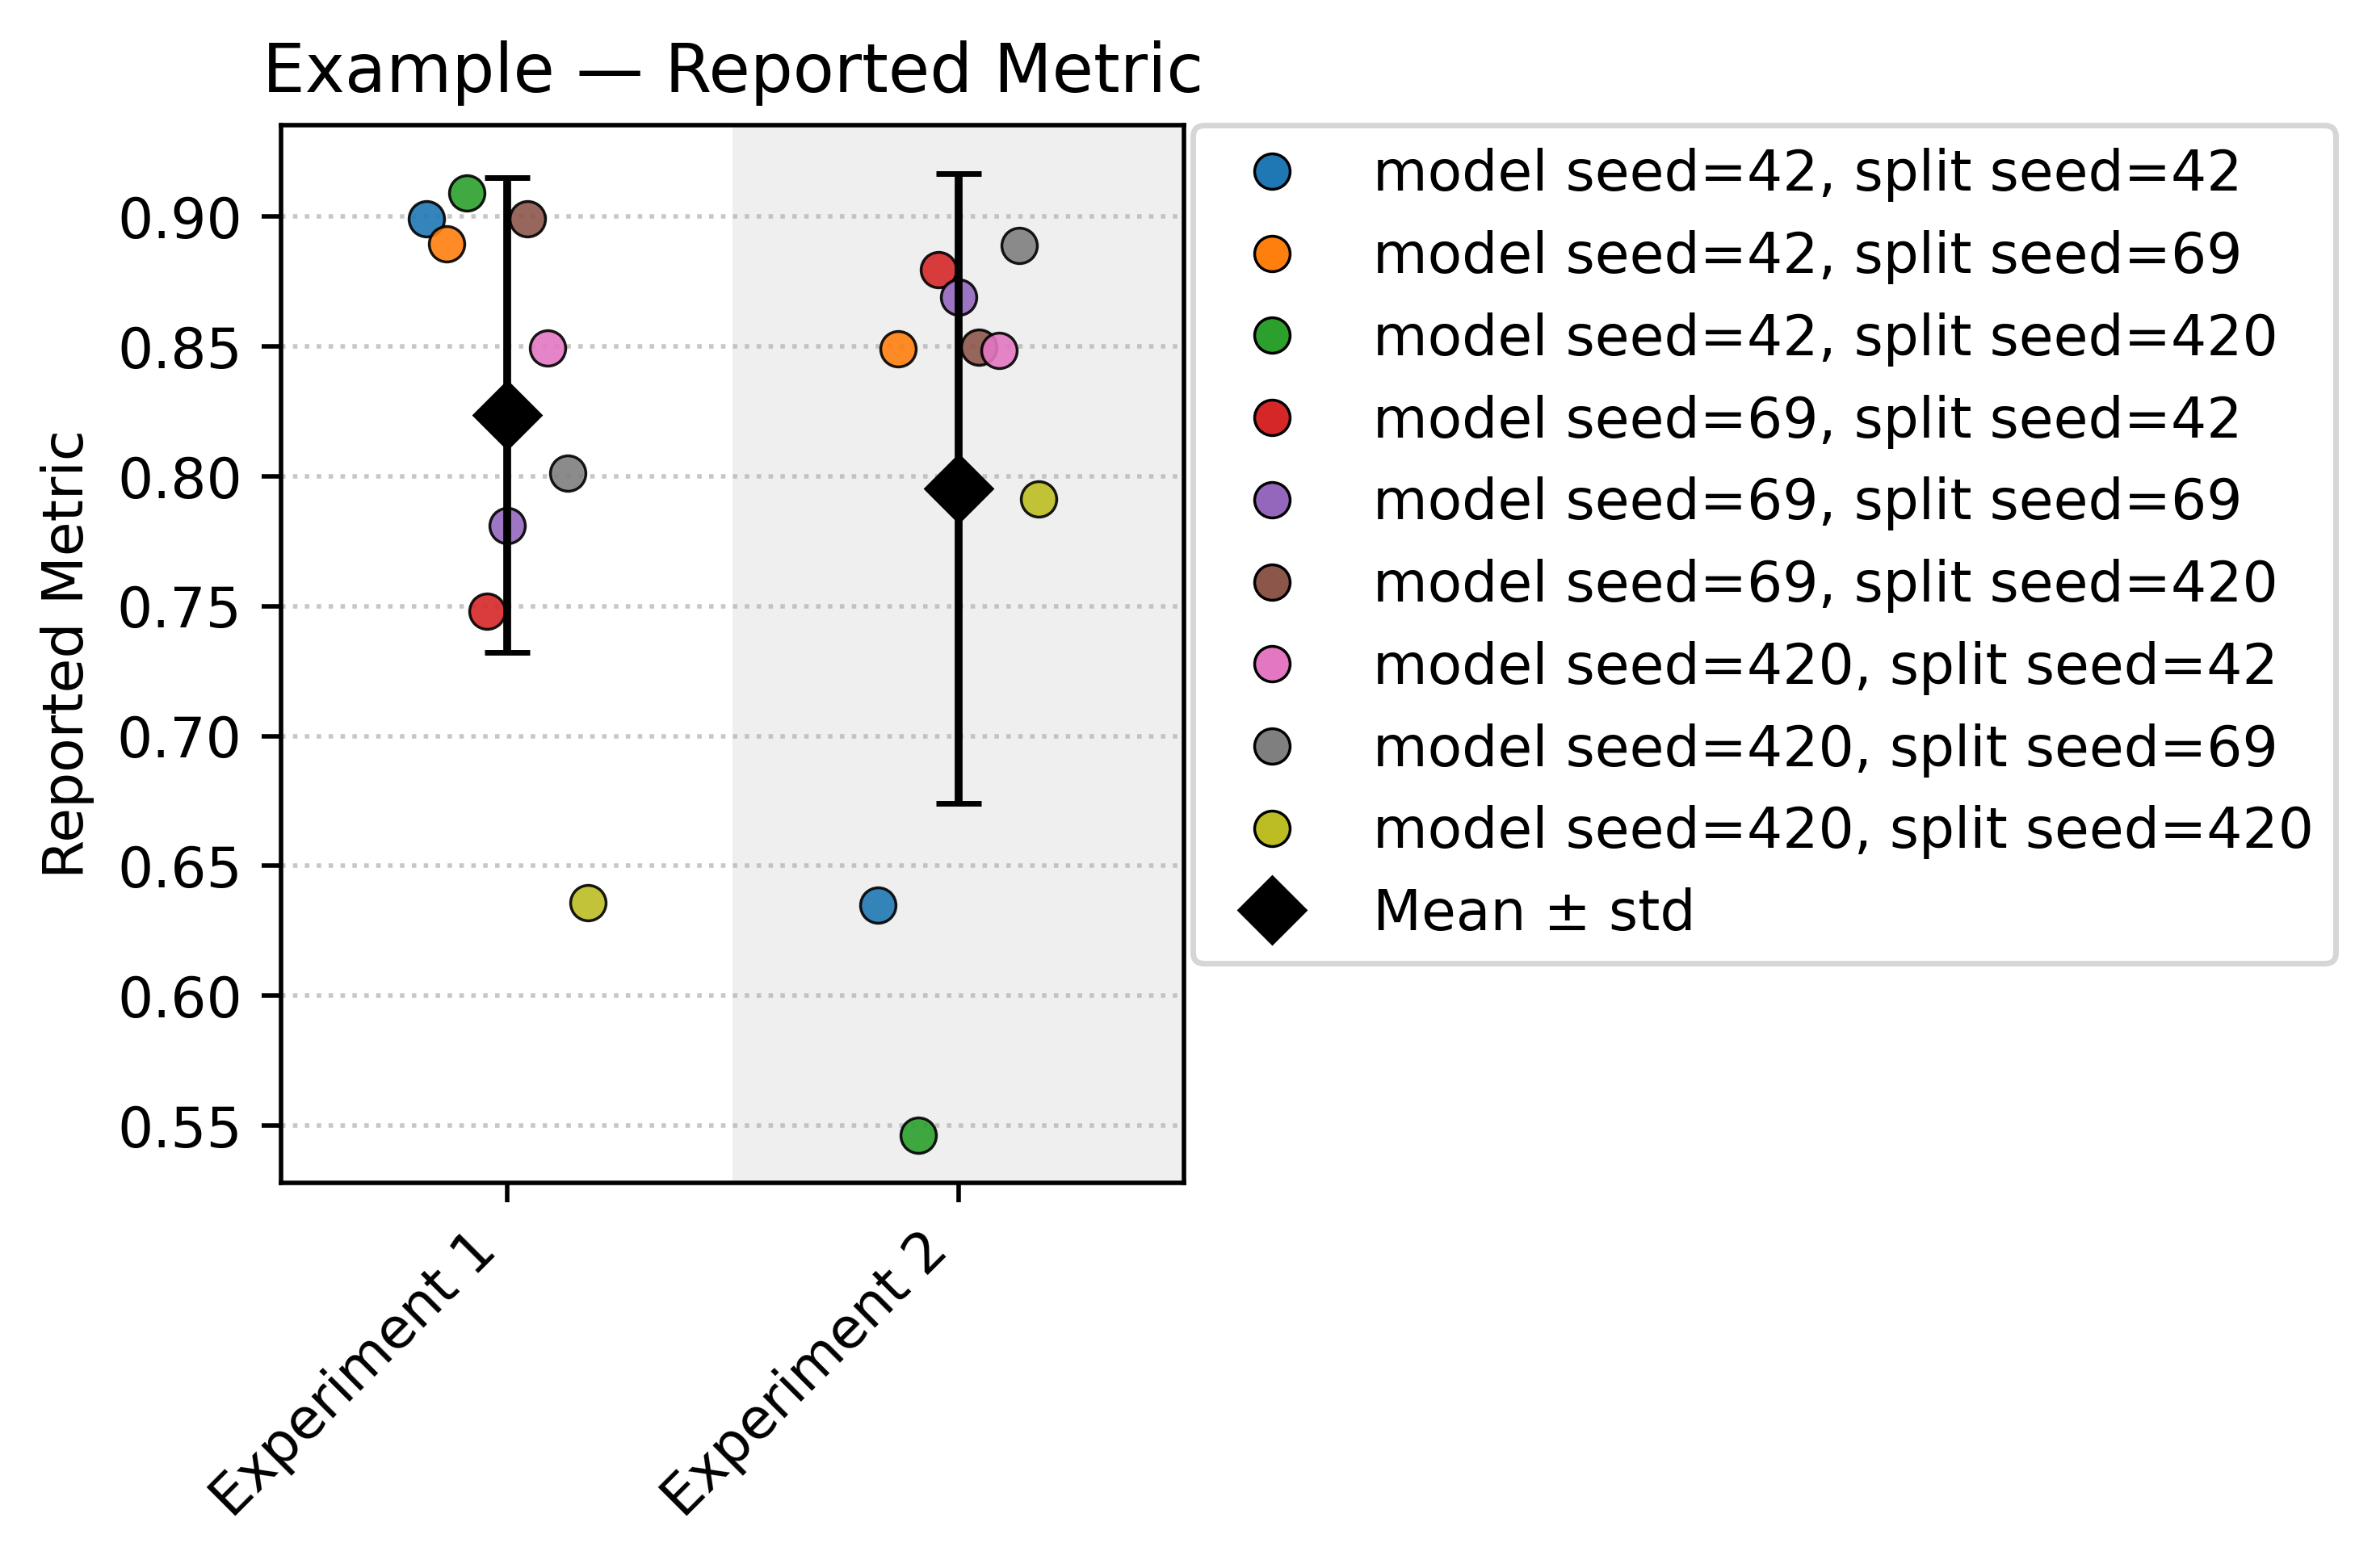
\includegraphics[width=0.7\textwidth]{chapters/6-experiments/bm_example.png}
    \caption{Benchmark/Experiment report example plot. Each dot is its own training run for one specific seed combination, which can be directly compared across different experiments 1 and 2.}
    \label{fig:bm_example}
\end{figure}

This design makes it possible to assess not only average performance but also robustness with respect to both data partitioning and stochastic training effects.

\section{Experiment 1: Best Channel Study}
\label{sec:exp1_best_channel_study}

\subsection{Motivation}

The recorded dataset contains several different signal modalities, including force/torque, TCP pose, TCP velocity, joint pose, joint velocity, tool acceleration, per-joint current, and temperature. These channel groups differ strongly in physical meaning and in how directly they describe the insertion process. Since the later benchmark studies should be done with one fixed channel configuration, it is necessary to determine beforehand which channel groups provide the most informative input for the classification task.

To keep the search doable, the study was not designed a full evaluation of all possible channel subsets. Instead, it was structured as a two-stage procedure: first, each channel group was evaluated individually to identify promising signal sources and second, the strongest groups were combined in different ways to determine an effective multi-modal channel configuration.

\subsection{Methods}
% All training runs in this study had no dedicated test set. The dataset is always split randomly in training and validation sets according to split ratios defined in Section \ref{subsec:train_val_test_splits}.
\paragraph{Stage 1: Individual channel-group tests}
In the first stage, each recorded channel group was evaluated individually using the \texttt{Base} PatchTST configuration introduced in \tabref{tab:patchtst_hyperparameters}. The investigated groups were:
\begin{itemize}
    \item F/T (\texttt{FT}),
    \item TCP pose (\texttt{TCP\_POS}),
    \item TCP velocity (\texttt{TCP\_VEL}),
    \item Joint pose (\texttt{JOINT\_POS}),
    \item Joint velocity (\texttt{JOINT\_VEL}),
    \item Tool acceleration from internal accelerometer (\texttt{TOOL\_ACC}),
    \item Current consumption per joint (\texttt{CURRENT}),
    \item Temperature per joint (\texttt{TEMP}).
\end{itemize}

% The purpose of this stage was to obtain an initial ranking of the channel groups under a common training setup. This screening step is computationally efficient and provides a first indication of which modalities are informative on their own. In particular, it helps distinguish directly interaction-related signals, such as force/torque, from more indirect state-related or actuator-related signals, such as TCP pose or current.

\paragraph{Stage 2: Combination study of the best groups}

Based on the results of the individual tests, the best-performing channel groups were selected. The main goal of this second stage was to determine whether complementary information from multiple modalities improves classification performance beyond what is achievable with any single group alone.

The combination study focused on the groups that showed the highest validation balanced accuracy in the first stage. These were:
\begin{itemize}
    \item F/T,
    \item TCP pose,
    \item Joint velocity,
    \item Current consumption.
\end{itemize}

These groups were then combined in all $4\times4=16$ possible ways, resulting in two-, three-, and four-group configurations. The second stage was evaluated with the larger \texttt{Big} PatchTST configuration, since the combined inputs increase the input dimensionality and may benefit from higher model capacity. The tested combinations are summarized by the result plots and by the channel-combination overview in \figref{fig:channel_combination_overview}.

\paragraph{Training and evaluation protocol}

No dedicated test set was used in this study. Instead, all runs were trained on a training split and compared on the validation split only. This is appropriate because the best channel study serves as an exploratory model-selection step before the actual benchmark experiments.

All configurations were trained repeatedly using the same combinations of model seed and split seed defined in Section \ref{sec:reporing_of_experiments}. The results were compared primarily using validation balanced accuracy. Validation loss is reported as well and provides an additional view on the calibration and stability of the models classifications. The main decision criterion for selecting the final channel configuration was validation balanced accuracy, while validation loss was used to support the interpretation of trade-offs between candidate configurations.

\subsection{Results}
\label{sec:best_channel_study_results}

\paragraph{Stage 1: Individual channel groups tests}

The results of the individual channel-group tests are shown in \figref{fig:best_channel_single_val_bal_acc} and \figref{fig:best_channel_single_val_loss}.

\begin{figure}[htpb]
    \centering
    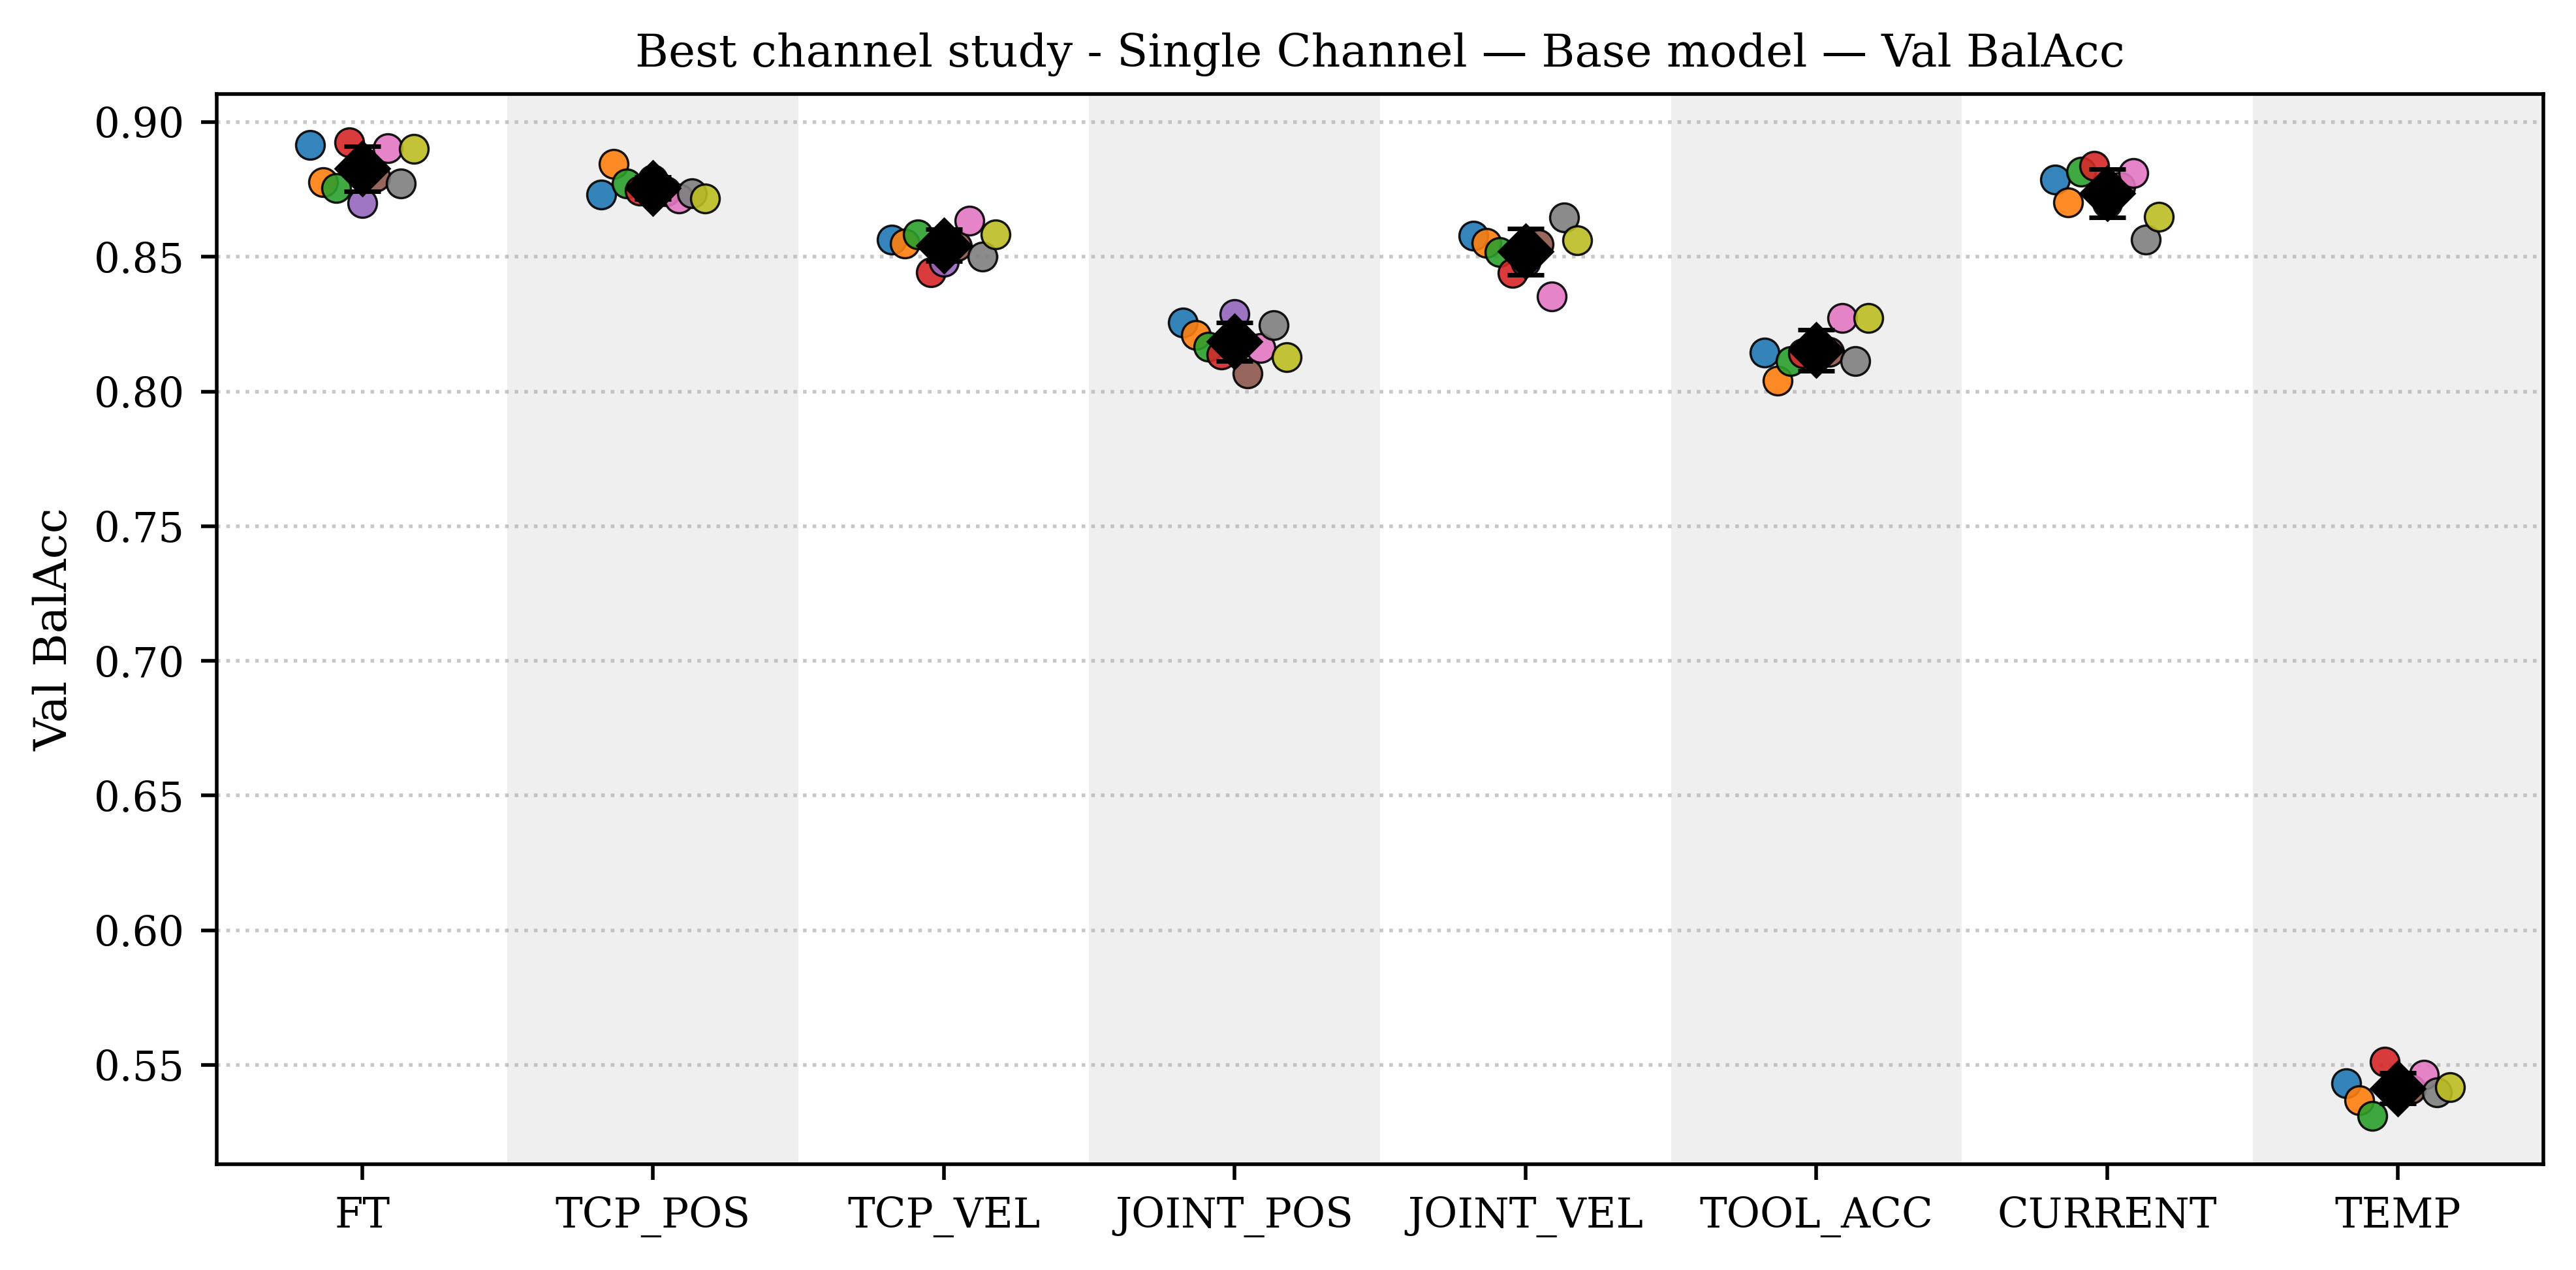
\includegraphics[width=1.0\textwidth]{chapters/6-experiments/single_channel_bal_acc.png}
    \caption{Validation balanced accuracy of the single channel-group tests with the \texttt{Base} model.}
    \label{fig:best_channel_single_val_bal_acc}
\end{figure}

\begin{figure}[htpb]
    \centering
    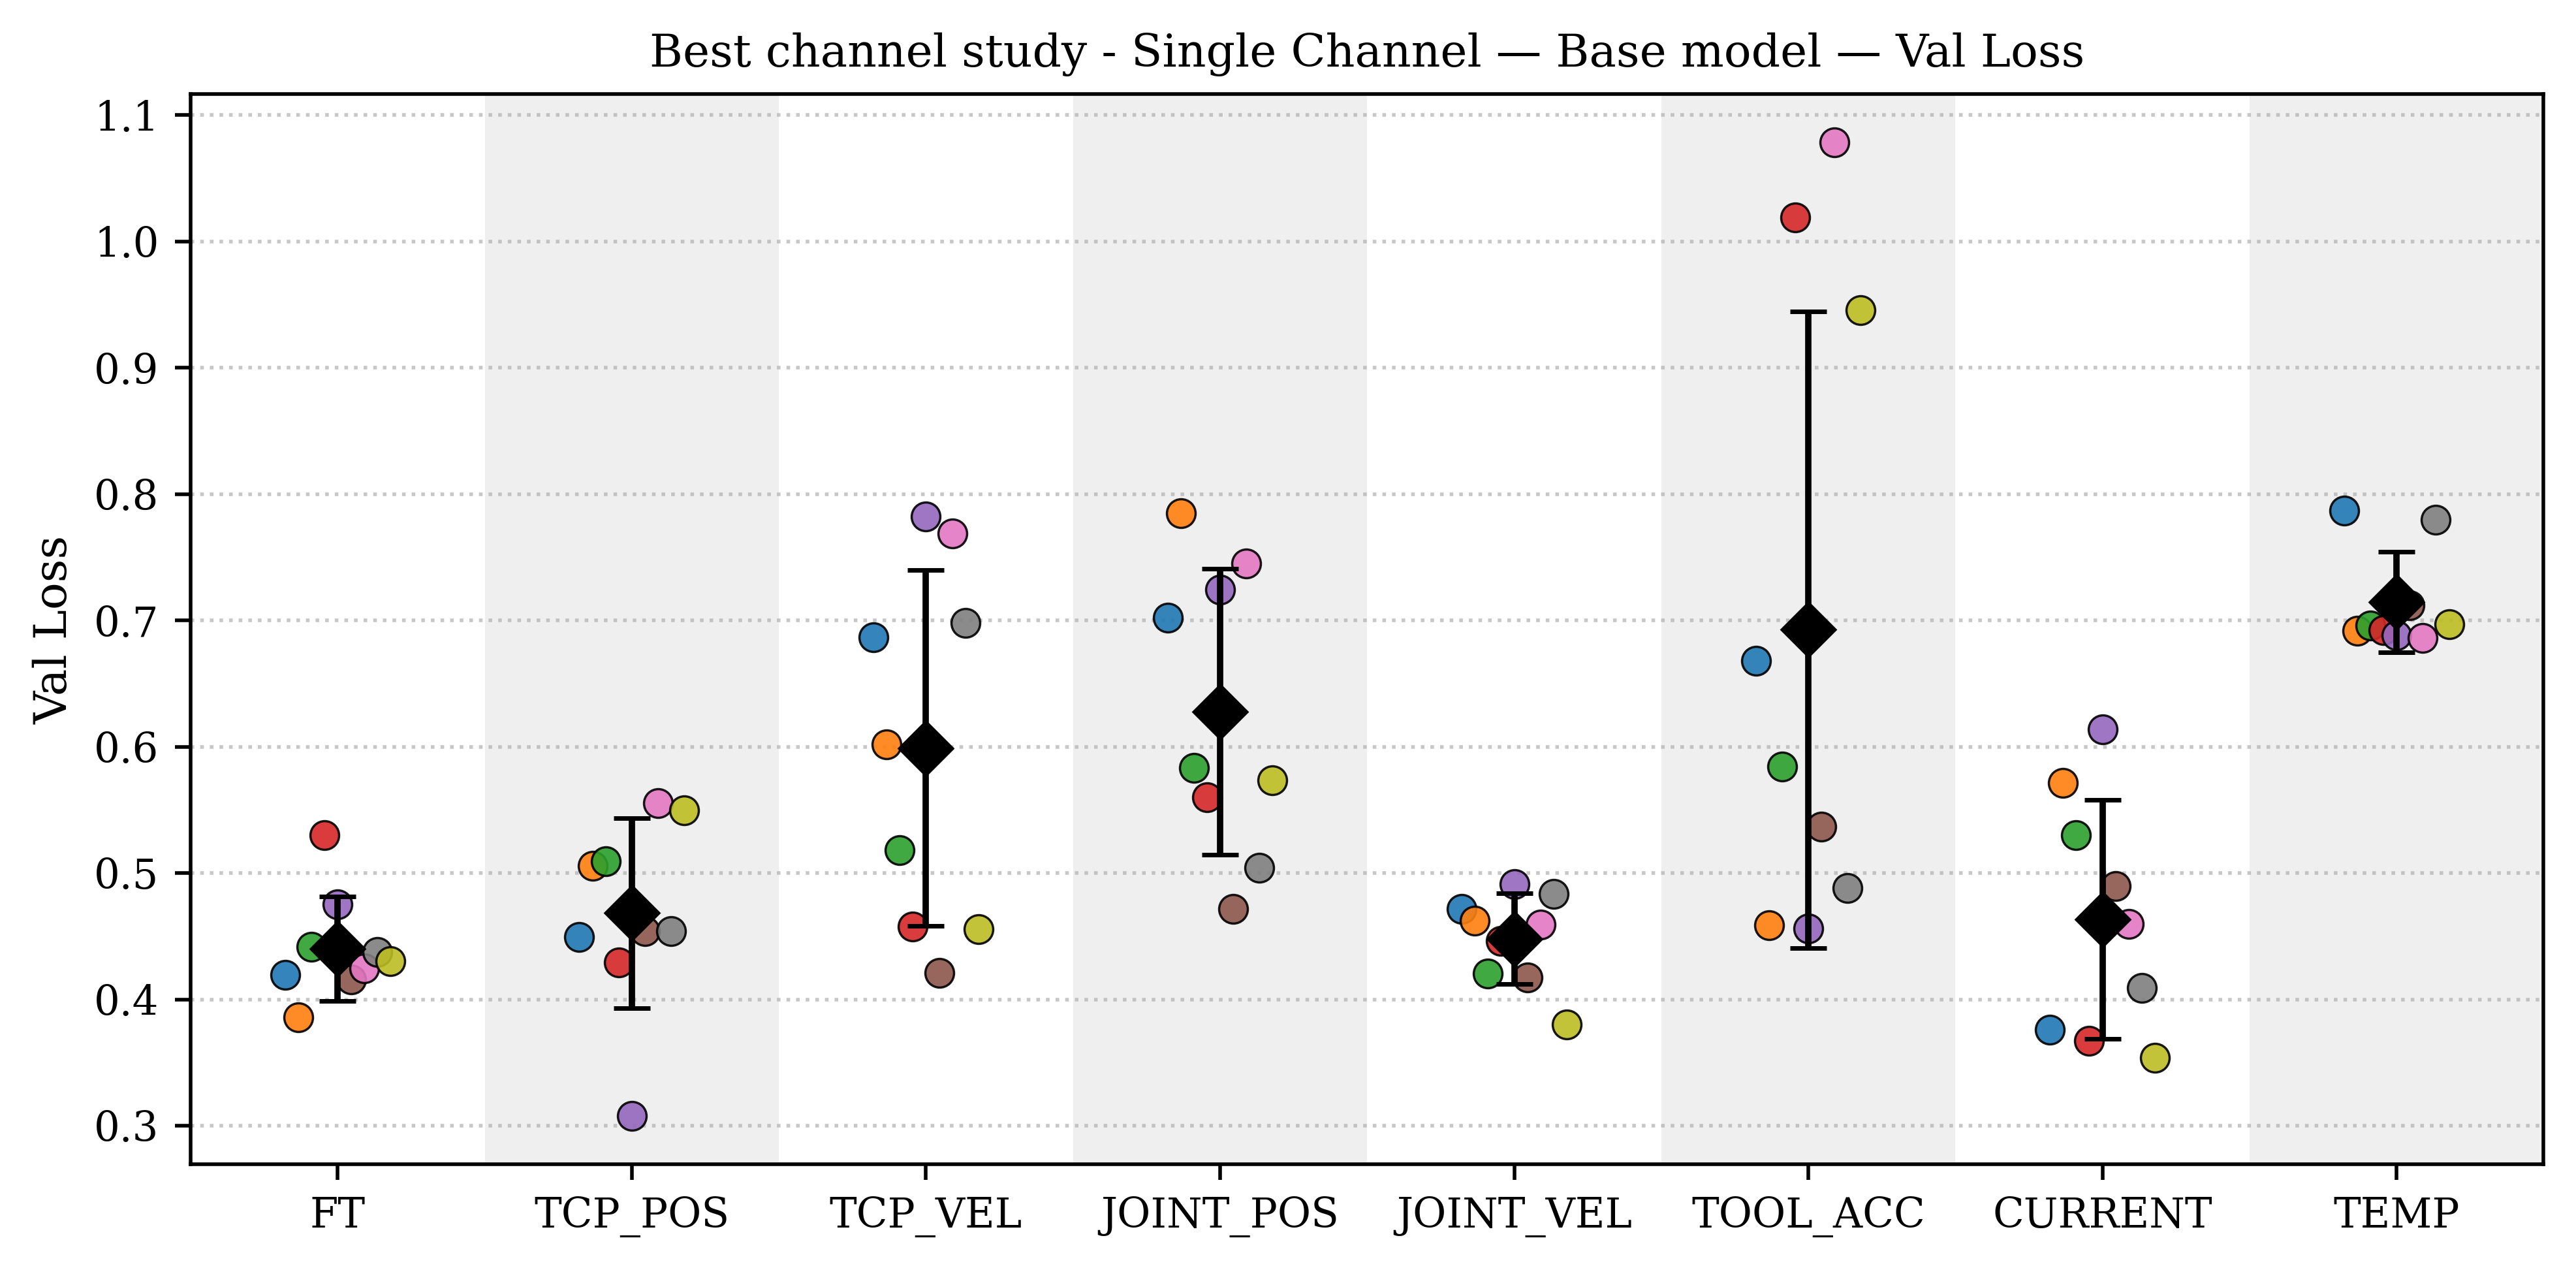
\includegraphics[width=1.0\textwidth]{chapters/6-experiments/single_channel_val_loss.png}
    \caption{Validation loss of the single channel-group tests with the \texttt{Base} model.}
    \label{fig:best_channel_single_val_loss}
\end{figure}

Several important observations can be made from these results. First, force/torque data provides the best standalone modality and is therefore the main candidate for the later stage 2 combination study. This is physically plausible, F/T describes the contact interaction during insertion most directly. Second, TCP pose and current also achieve comparatively high validation balanced accuracy, despite being more indirect measurements. This indicates that the insertion outcome is not encoded only in direct contact signals, but also in robot state and actuator-related signals. Third, joint velocity performs better than TCP velocity and tool acceleration, making it the more promising dynamic complement. Classification with temperature performs almost random and is therefore not considered further.

To summarize, the individual tests suggested that the most informative single groups are F/T, TCP pose, current, and joint velocity. These groups were therefore selected as the basis for the next stage of the study.

\paragraph{Stage 2: Combination study}

The results of the second-stage combination study are shown for the two-group configurations in \figref{fig:two_group_bal_acc} and \figref{fig:two_group_val_loss} and the three- and four-group configurations in \figref{fig:three_group_bal_acc} and \figref{fig:three_group_val_loss}. Here, different combinations of the strongest channel groups from Stage 1 were evaluated using the \texttt{Big} model.

\begin{figure}[htpb]
    \centering
    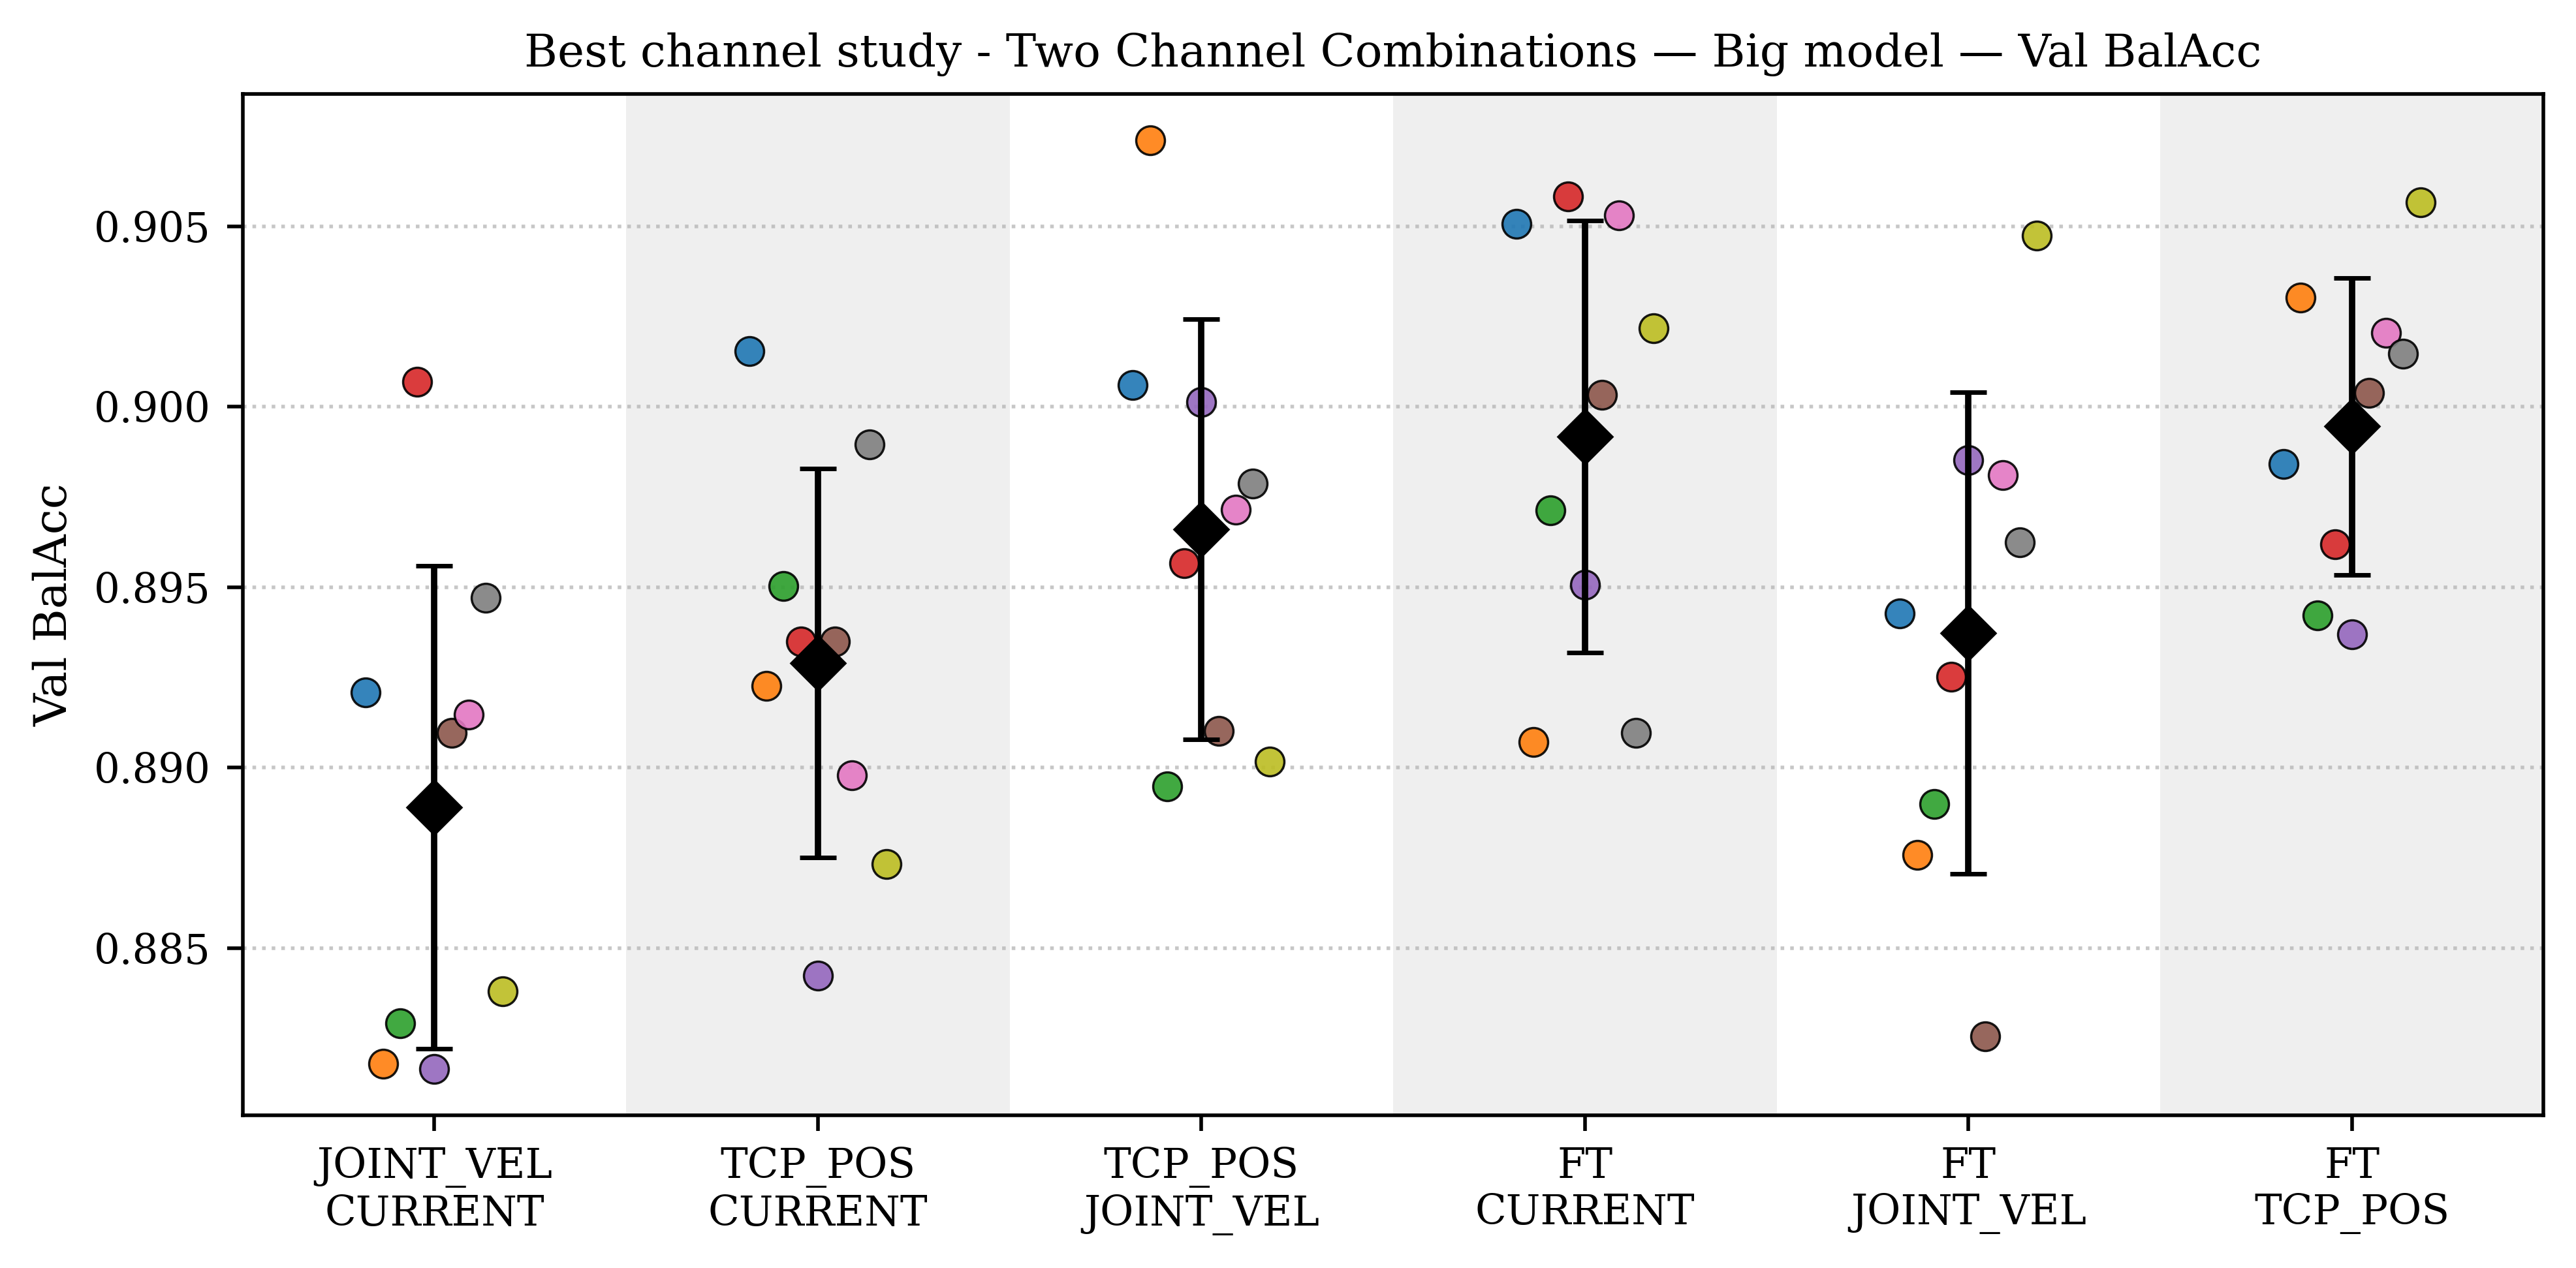
\includegraphics[width=1.0\textwidth]{chapters/6-experiments/two_channel_combos_bal_acc.png}
    \caption{Validation balanced accuracy of all two-group configurations evaluated with the \texttt{Big} model.}
    \label{fig:two_group_bal_acc}
\end{figure}

\begin{figure}[htpb]
    \centering
    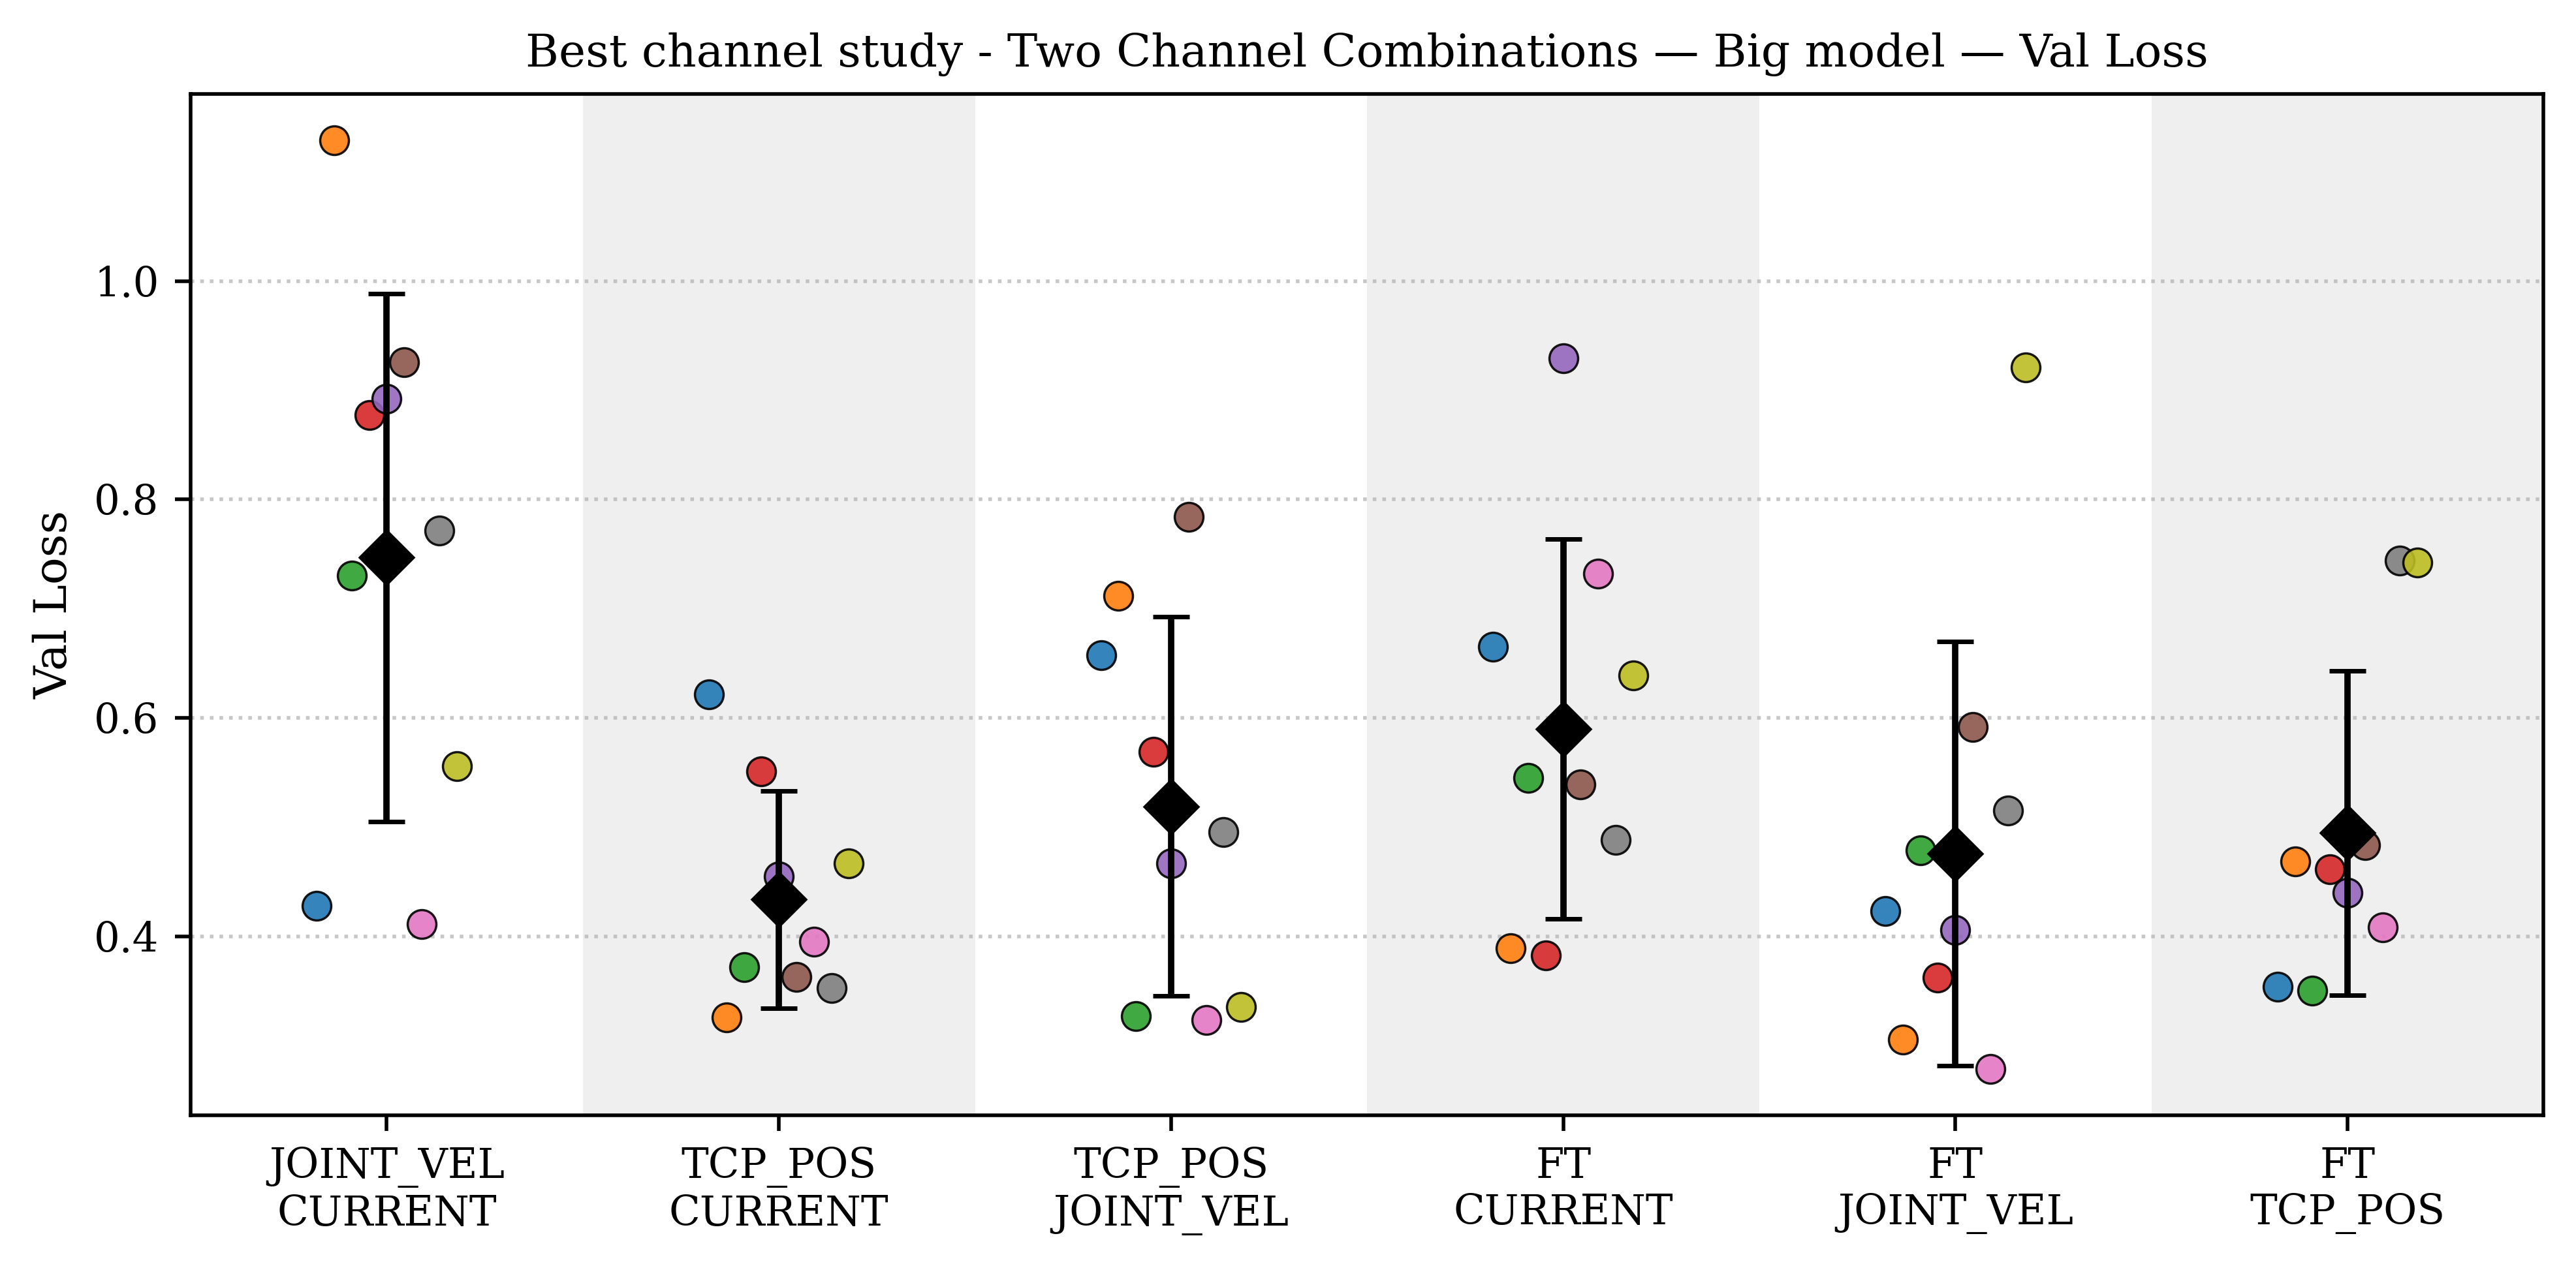
\includegraphics[width=1.0\textwidth]{chapters/6-experiments/two_channel_combos_val_loss.png}
    \caption{Validation loss of all two-group configurations evaluated with the \texttt{Big} model.}
    \label{fig:two_group_val_loss}
\end{figure}

\begin{figure}[htpb]
    \centering
    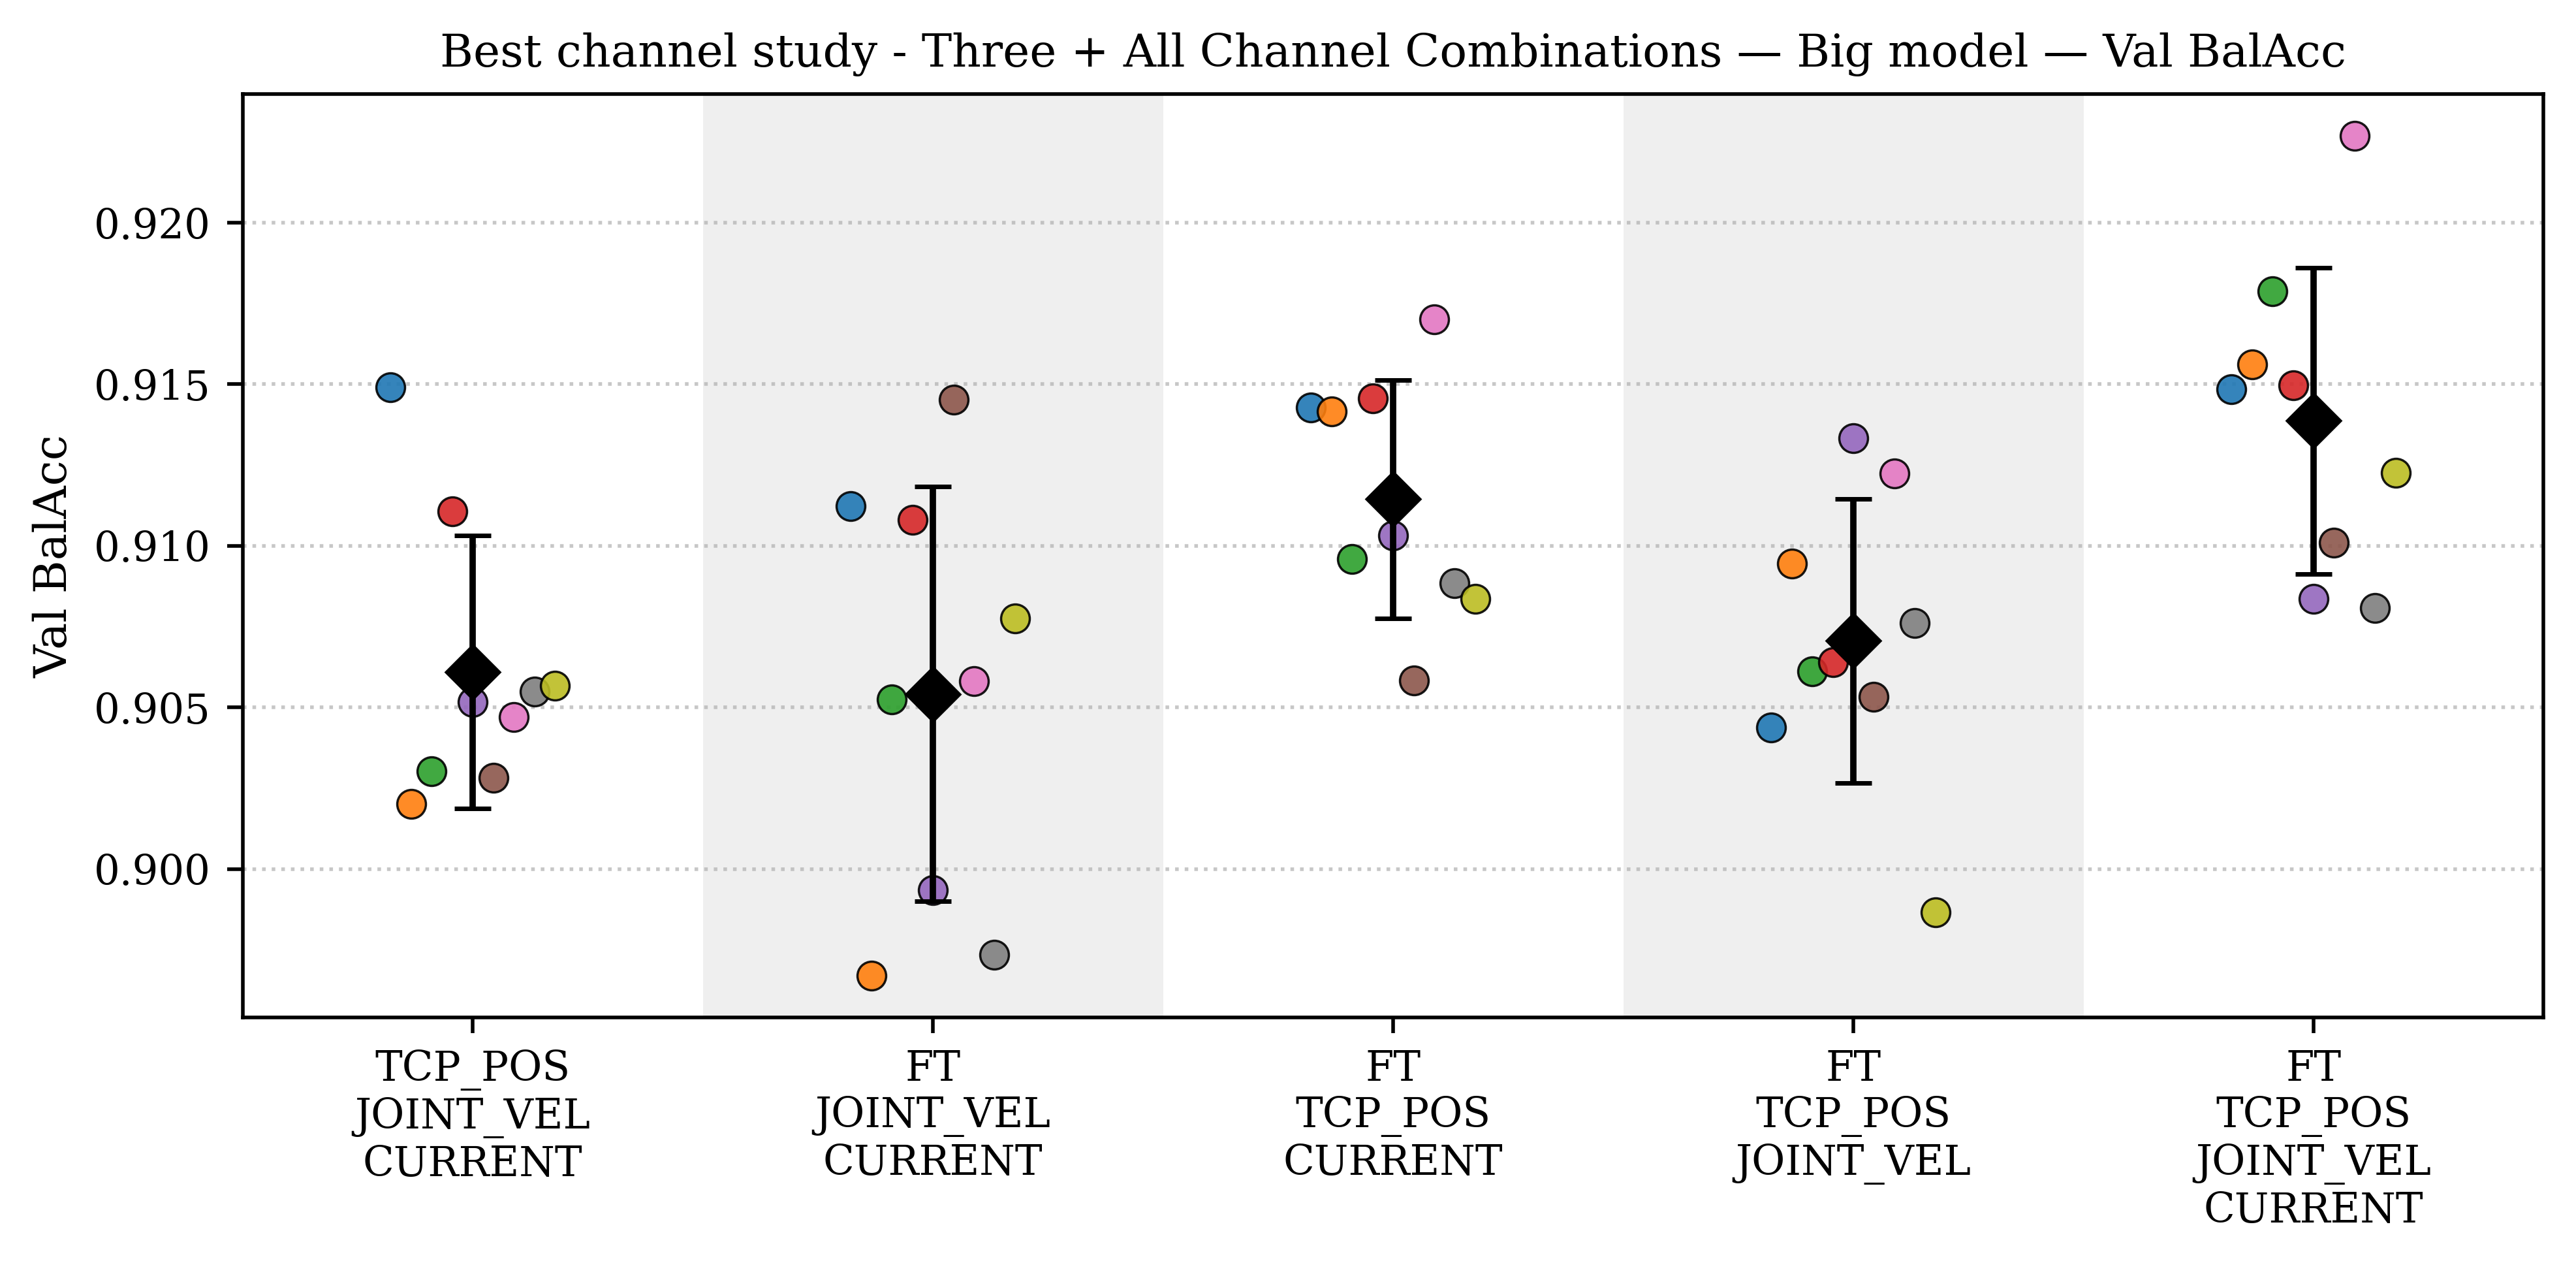
\includegraphics[width=1.0\textwidth]{chapters/6-experiments/three_channel_combos_bal_acc.png}
    \caption{Validation balanced accuracy of all three- and four-group configurations evaluated with the \texttt{Big} model.}
    \label{fig:three_group_bal_acc}
\end{figure}

\begin{figure}[htpb]
    \centering
    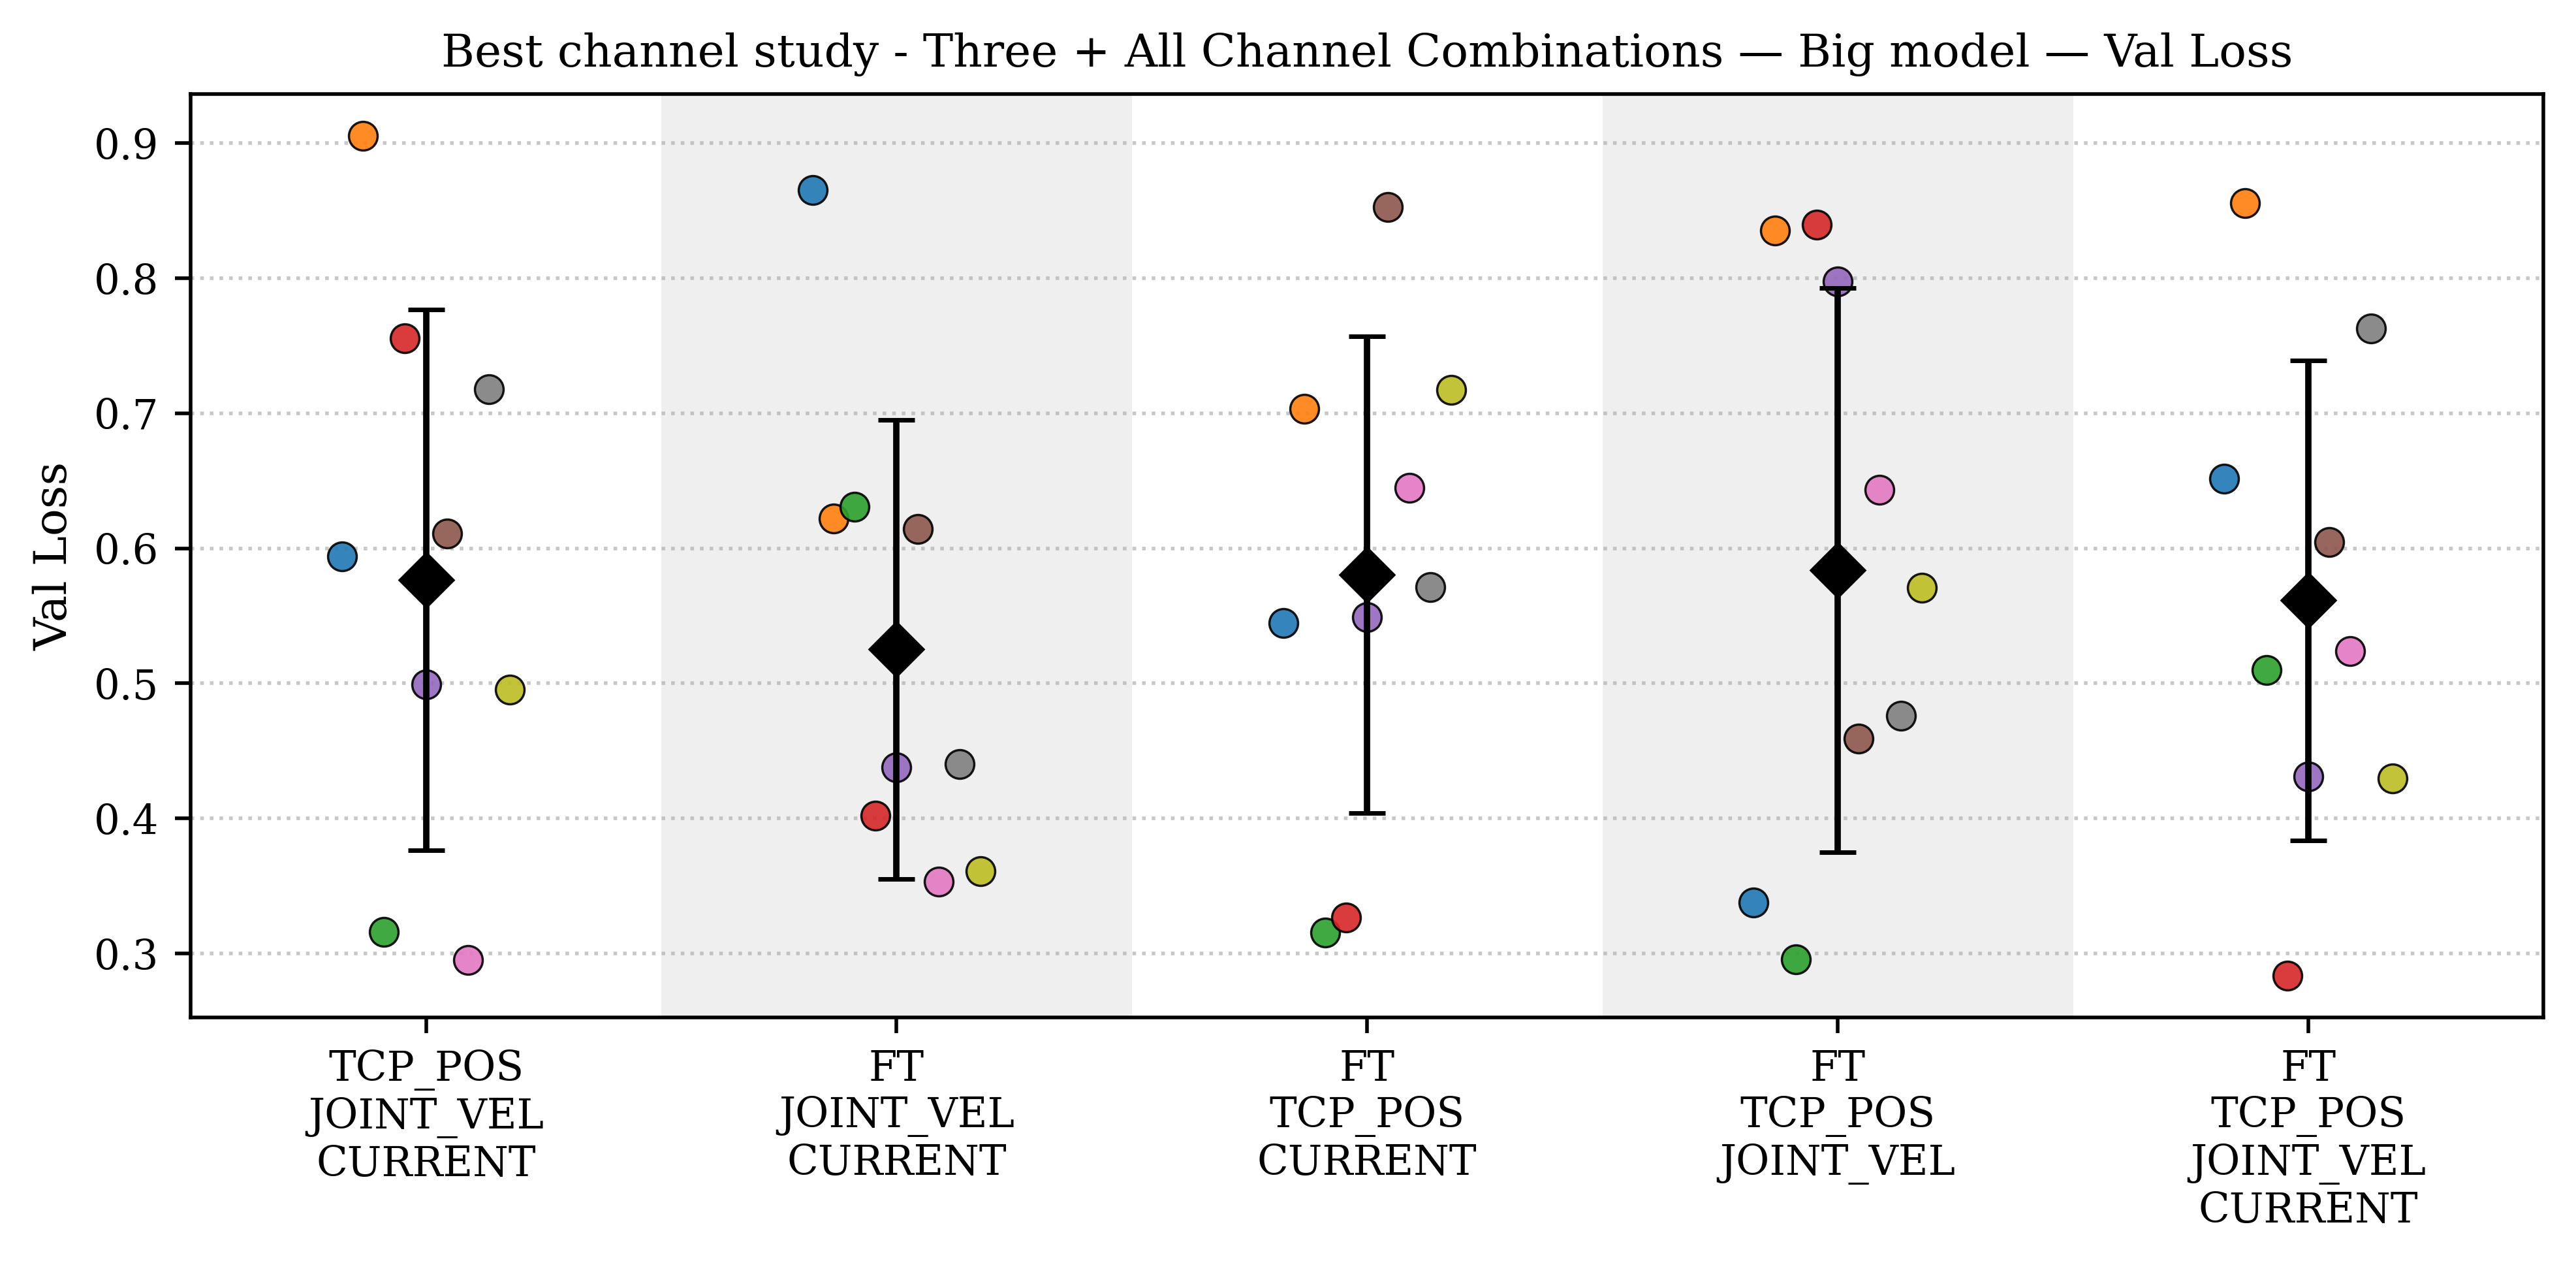
\includegraphics[width=1.0\textwidth]{chapters/6-experiments/three_channel_combos_val_loss.png}
    \caption{Validation loss of all three- and four-group configurations evaluated with the \texttt{Big} model.}
    \label{fig:three_group_val_loss}
\end{figure}

The most important result of this second stage is that combining multiple already good and complementary channel groups yields better validation performance than using them individually. In particular, the combination of F/T, current, TCP pose, and joint velocity achieved the best validation balanced accuracy among the tested combinations.

The plots also show that the addition current is particularly valuable. While it is not a direct contact measurement, it consistently improves the multi-modal configurations and therefore contributes relevant information for the classification task. TCP pose likewise provides useful information, which indicates that the robot state contains information correlated with successful and failed insertions. Joint velocity further improves the strongest combinations and appears to be more reliable than TCP velocity, because the validation loss is lower and much less spread.

\paragraph{Channel combination overview}

For completeness, \figref{fig:channel_combination_overview} summarizes the full set of evaluated channel configurations in a compact form. The figure shows for each configuration which channel groups were included and reports the corresponding validation metrics for the available \texttt{Base} and \texttt{Big} model runs.

\begin{figure}[htpb]
    \centering
    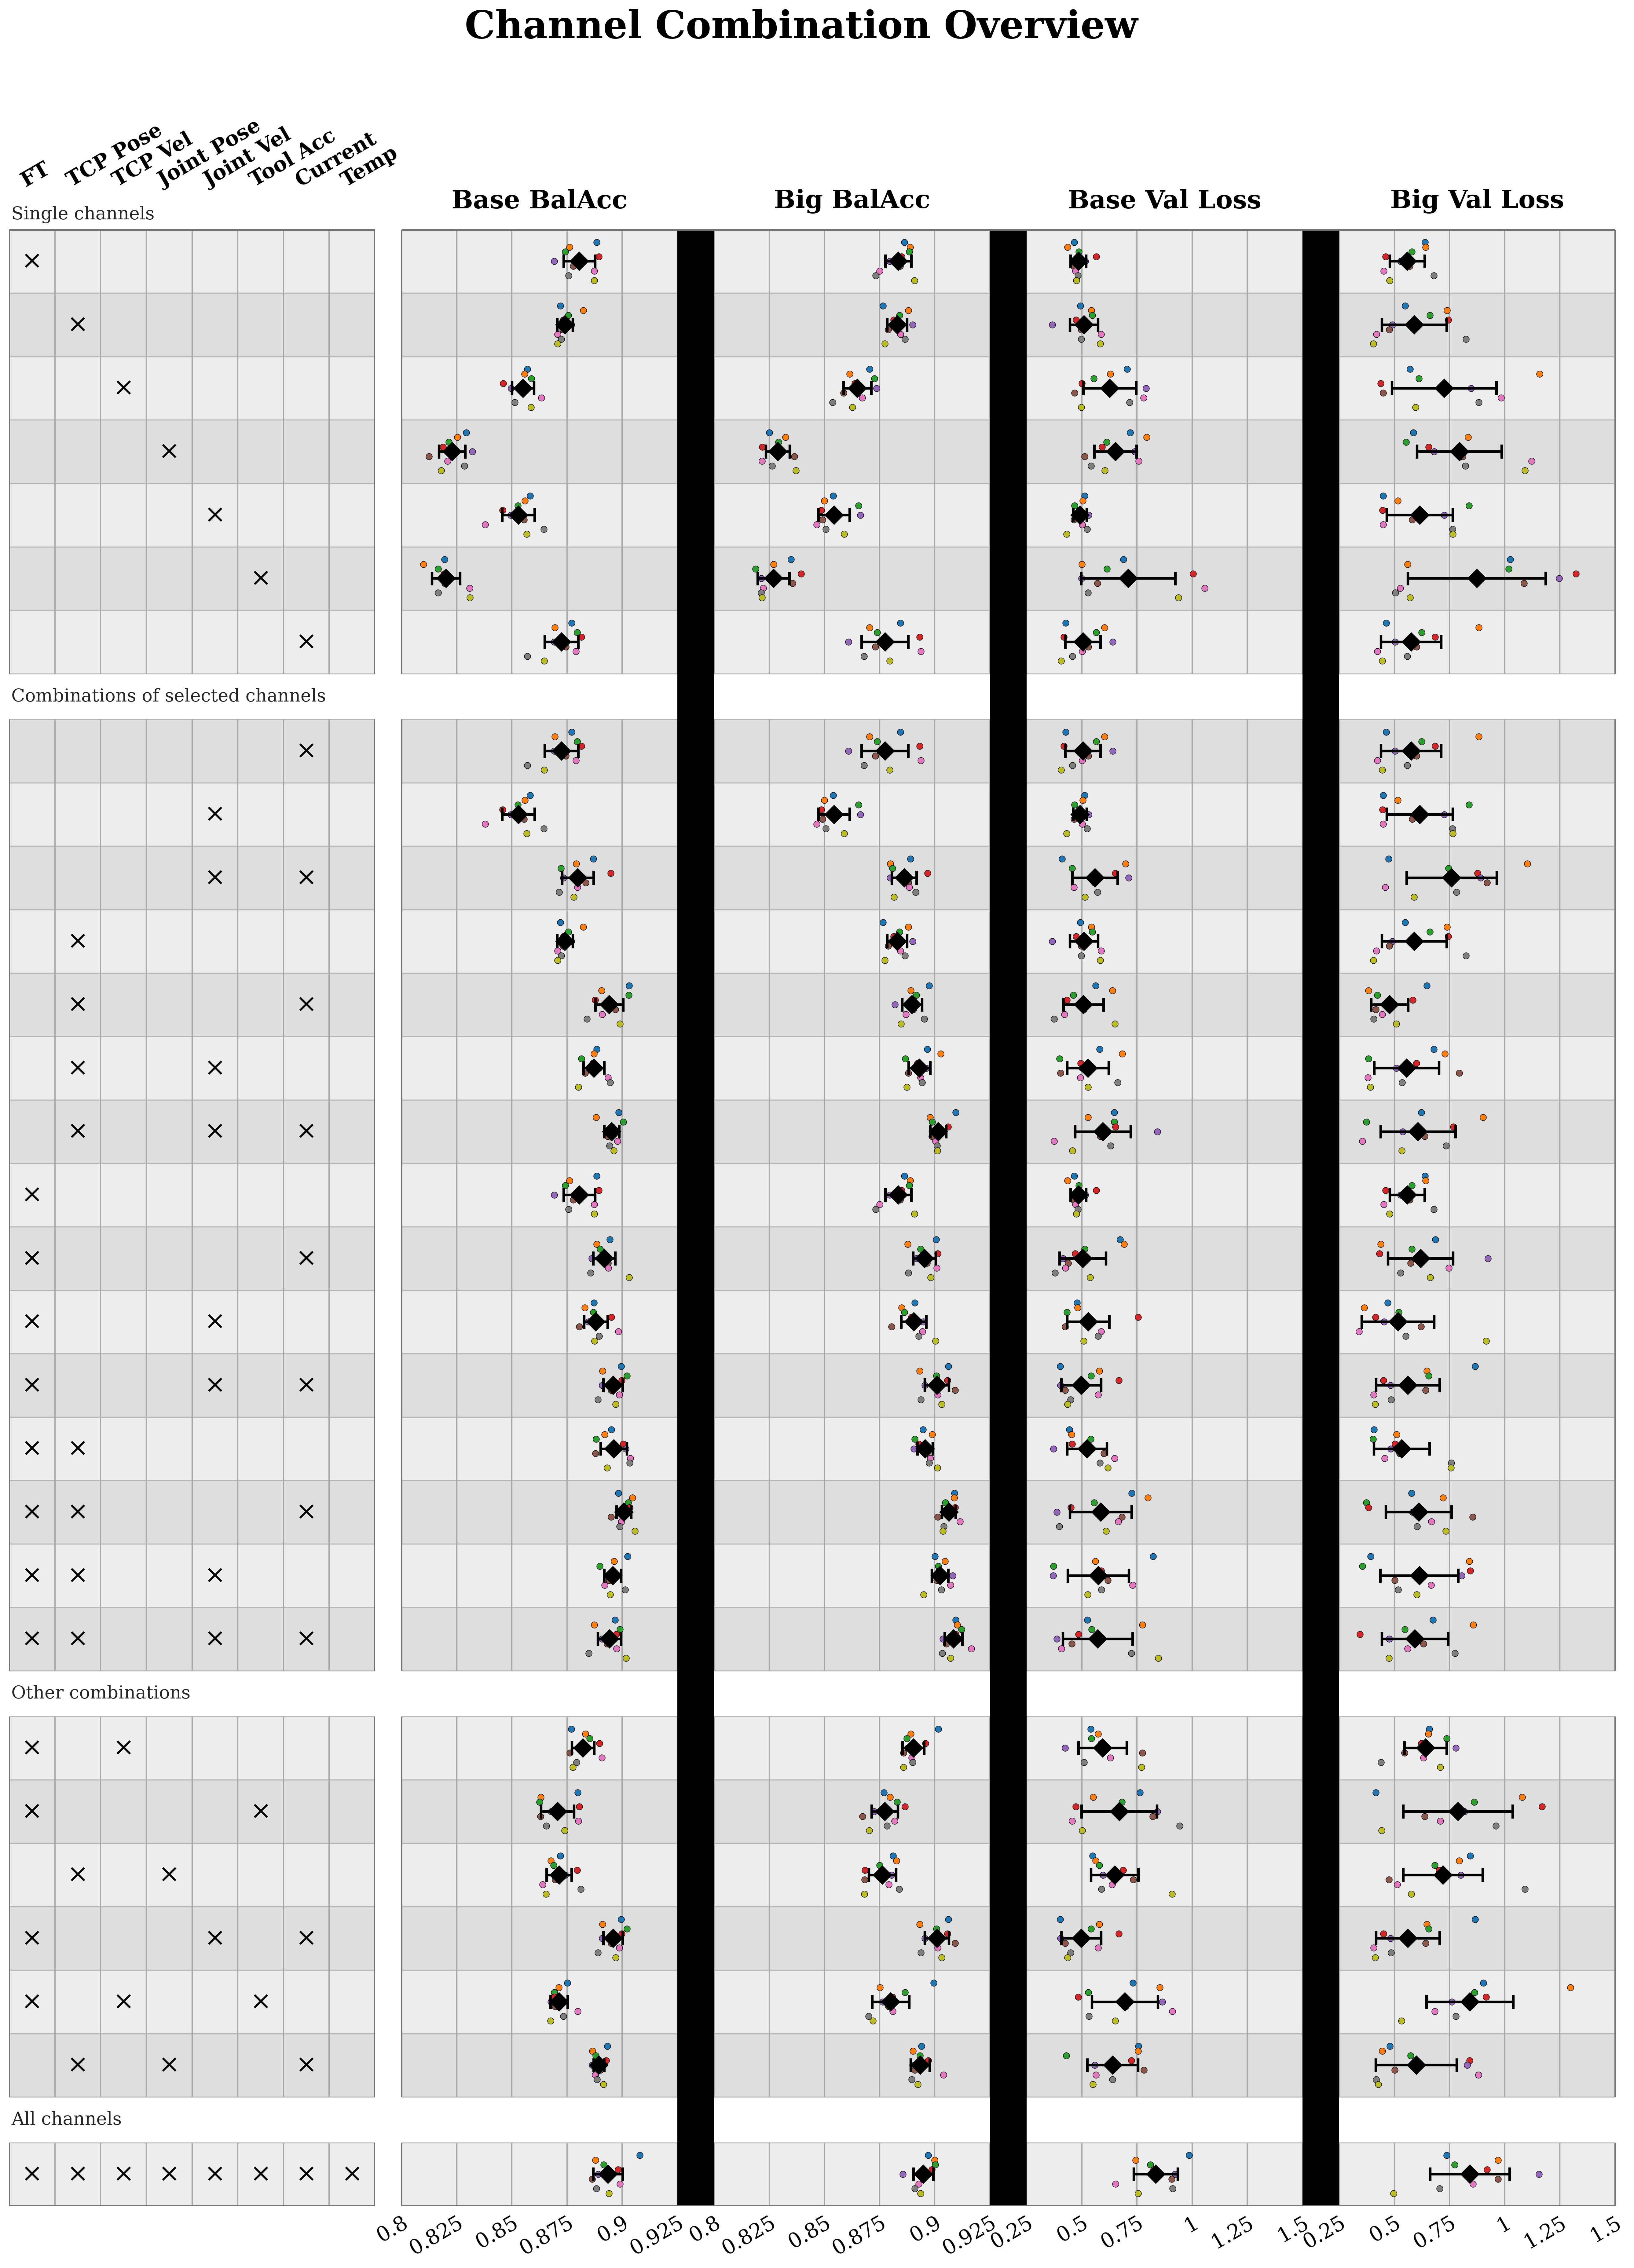
\includegraphics[width=1.0\textwidth]{chapters/6-experiments/channel_matrix_plot.png}
    \caption{Overview of the evaluated channel configurations. Crosses indicate which channel groups are included in each configuration. The corresponding validation balanced accuracy and validation loss for the available \texttt{Base} and \texttt{Big} runs are shown on the right. The temperature signal is not shown, because it heavily scews the plot.}
    \label{fig:channel_combination_overview}
\end{figure}

This overview makes the overall progression of the study transparent. It shows the initial single-group screening, the subsequent combination experiments, and the final selected multi-modal configurations in one figure.

\paragraph{Final channel selection}

Based on the two-stage study, the channel configuration selected for the remainder of the thesis consists of the following four groups:
\begin{itemize}
    \item F/T,
    \item TCP pose,
    \item joint velocity,
    \item and current.
\end{itemize}

This selection is motivated primarily by the highest observed validation balanced accuracy in the combination study, supported by competitive validation loss. It therefore represents the best overall trade-off among the tested configurations and is carried forward into the later benchmark studies.

\subsection{Discussion and Conclusion}

The best channel study leads to three main conclusions. First, F/T is the best single channel group, but the best overall results are achieved when it is combined with additional modalities. Successful insertion classification is therefore not encoded in one signal group alone.

Second, current and TCP pose provide substantial additional information, even though they are more indirect than F/T.

Third, the best-performing configuration combines complementary information: contact interaction through F/T, actuator load through current consumption, robot state through TCP pose, and motion dynamics through joint velocity.

Overall, the results show that robust insertion-success classification benefits from multi-modal input. Therefore, the combination of F/T, TCP pose, joint velocity, and current is used in the remainder of the thesis.







\section{Experiment 2: PatchTST Benchmark Evaluation}
\subsection{Benchmark 1: Test on Mixed Split}
\label{sec:sq2_mixed_split}

Benchmark 1 implements an in-distribution evaluation with a random mixed split of the dataset. The full data pool is divided into a training, validation subsets, with the testset drawn from the domain \texttt{BM1} defined in \tabref{tab:bm1_domains} using the split ratios defined in Section \ref{subsec:train_val_test_splits}. This Benchmark specifically uses the first split strategy as described in the mentioned section.

As a result, the test set contains unseen insertion attempts, but not unseen experimental conditions. This benchmark therefore quantifies the model's performance when training and test data are drawn from the same overall distribution. The evaluated model configurations are the ones selected in the best channel study, and each configuration is trained and evaluated over the full set of seed combinations defined in the common training procedure in Section \ref{sec:reporing_of_experiments}.

\begin{table}[htbp]
    \centering
    \caption{Benchmark 1 Domains.}
    \label{tab:bm1_domains}
    \begin{tabular}{lllll}
        \toprule
        \textbf{Domain} & \textbf{\texttt{batch}} & \textbf{\texttt{rod\_type}} & \textbf{\texttt{tolerance}} & \textbf{\texttt{gripper\_type}} \\
        \midrule
        \texttt{BM1} & \texttt{None} & \texttt{None} & \texttt{None} & \texttt{None}\\
        \bottomrule
    \end{tabular}
\end{table}

\subsection{Benchmark 2: Test on Individual Hole}
\label{sec:sq3_individual_hole}

Benchmark 2 implements a leave-one-hole-out evaluation. In each run, all samples belonging to one domain from \texttt{BM2\_Hole\_1} to \texttt{BM2\_Hole\_9}, as defined in \tabref{tab:bm2_domains}, are assigned exclusively to the test set. The remaining data is used to form the training and validation set according to the common split procedure described in Section \ref{subsec:train_val_test_splits}.

Thus, the test set contains unseen insertion attempts from one domain that is completely absent from training. This benchmark evaluates whether the classifier generalizes to a new hole domains rather than only to new samples from already observed insertions. The evaluated hole domains are corresponding to the nine labeled holes shown in \figref{fig:taskboard_holes}, and each benchmark domain is evaluated for the selected model configurations over the full set of seed combinations.

\begin{table}[htbp]
    \centering
    \caption{Benchmark 2 Domains.}
    \label{tab:bm2_domains}
    \begin{tabular}{lllll}
        \toprule
        \textbf{Domain} & \textbf{\texttt{batch}} & \textbf{\texttt{rod\_type}} & \textbf{\texttt{tolerance}} & \textbf{\texttt{gripper\_type}} \\
        \midrule
        \texttt{BM2\_big\_1} & \texttt{None} & \texttt{big\_rod} & \texttt{0.1} & \texttt{None}\\
        \texttt{BM2\_big\_2} & \texttt{None} & \texttt{big\_rod} & \texttt{0.2} & \texttt{None}\\
        \texttt{BM2\_big\_3} & \texttt{None} & \texttt{big\_rod} & \texttt{0.3} & \texttt{None}\\

        \texttt{BM2\_small\_1} & \texttt{None} & \texttt{small\_rod} & \texttt{0.1} & \texttt{None}\\
        \texttt{BM2\_small\_2} & \texttt{None} & \texttt{small\_rod} & \texttt{0.2} & \texttt{None}\\
        \texttt{BM2\_small\_3} & \texttt{None} & \texttt{small\_rod} & \texttt{0.3} & \texttt{None}\\

        \texttt{BM2\_rect\_1} & \texttt{None} & \texttt{rect\_rod} & \texttt{0.1} & \texttt{None}\\
        \texttt{BM2\_rect\_2} & \texttt{None} & \texttt{rect\_rod} & \texttt{0.2} & \texttt{None}\\
        \texttt{BM2\_rect\_3} & \texttt{None} & \texttt{rect\_rod} & \texttt{0.3} & \texttt{None}\\
        \bottomrule
    \end{tabular}
\end{table}

\begin{figure}[htbp]
    \centering
    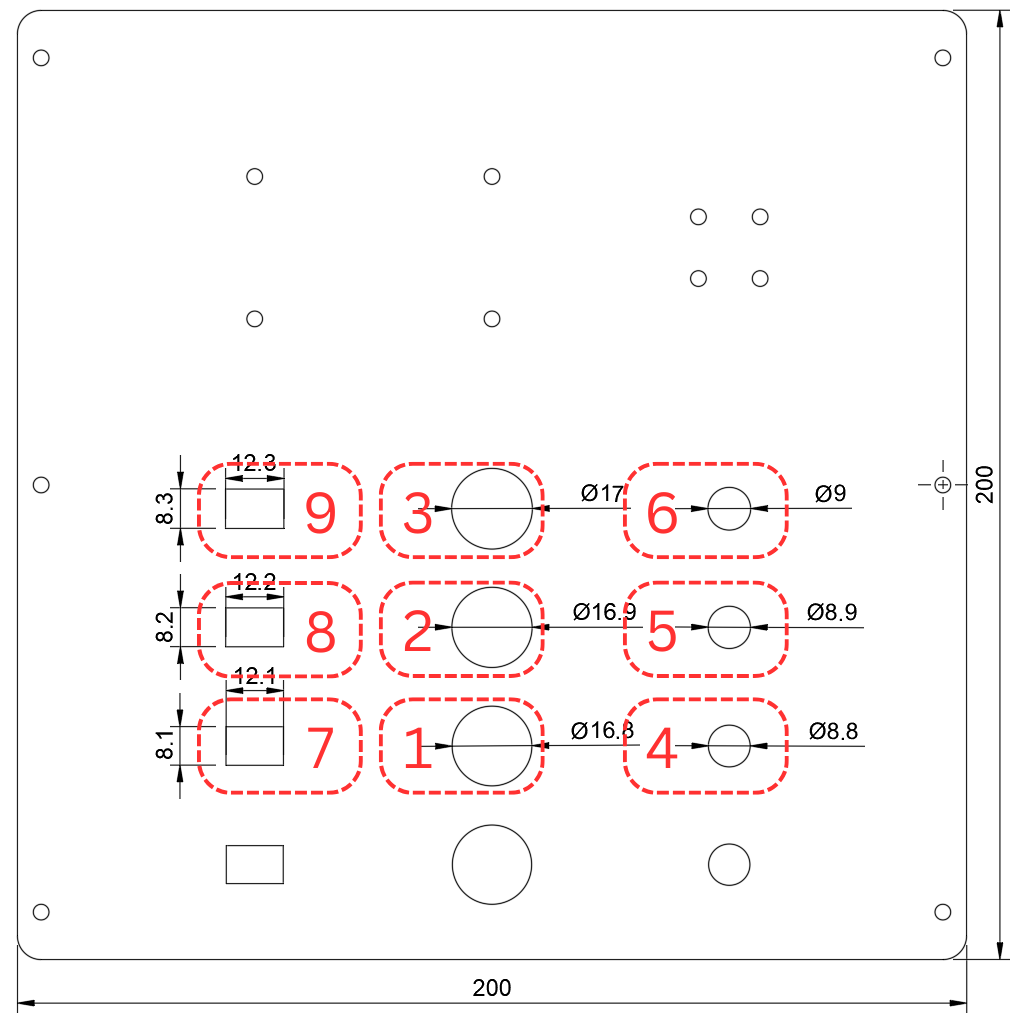
\includegraphics[width=0.6\linewidth]{chapters/6-experiments/bm1_taskboard.png}
    \caption{Schematic drawing of the insertion taskboard. The nine hole domains used in Benchmark 2 are labeled from 1 to 9. Each hole corresponds to one specific domain, defined in \tabref{tab:bm2_domains}. 1: \texttt{BM2\_Hole\_1} $\dots$ 9: \texttt{BM2\_Hole\_9}.}
    \label{fig:taskboard_holes}
\end{figure}

\subsection{Benchmark 3: Test on Held-Out Group}
\label{sec:sq4_held_out_group}

Benchmark 3 evaluates generalization under broader distribution shifts by holding out entire groups of samples from training and validation and using them exclusively for testing. These group domains are defined in \tabref{tab:bm3_domains}.

For each benchmark domain, all samples belonging to the selected domain group are assigned to the test set, while the remaining data is split into training and validation sets according to the common procedure described in Section \ref{subsec:train_val_test_splits}.

The held-out rod and held-out tolerance domains are shown in \figref{fig:heldout_groups}, while the gripper- and batch-based splits are evaluated in the same way.

\begin{table}[htbp]
    \centering
    \caption{Benchmark 3 Domains.}
    \label{tab:bm3_domains}
    \begin{tabular}{lllll}
        \toprule
        \textbf{Domain} & \textbf{\texttt{batch}} & \textbf{\texttt{rod\_type}} & \textbf{\texttt{tolerance}} & \textbf{\texttt{gripper\_type}} \\
        \midrule

        \texttt{BM3\_batch\_1} & \texttt{batch\_1} & \texttt{None} & \texttt{None} & \texttt{None}\\
        \texttt{BM3\_batch\_2} & \texttt{batch\_2} & \texttt{None} & \texttt{None} & \texttt{None}\\
        \texttt{BM3\_batch\_3} & \texttt{batch\_3} & \texttt{None} & \texttt{None} & \texttt{None}\\

        \texttt{BM3\_big} & \texttt{None} & \texttt{big\_rod} & \texttt{None} & \texttt{None}\\
        \texttt{BM3\_small} & \texttt{None} & \texttt{small\_rod} & \texttt{None} & \texttt{None}\\
        \texttt{BM3\_rect} & \texttt{None} & \texttt{rect\_rod} & \texttt{None} & \texttt{None}\\

        \texttt{BM3\_tol\_1} & \texttt{None} & \texttt{None} & \texttt{0.1} & \texttt{None}\\
        \texttt{BM3\_tol\_2} & \texttt{None} & \texttt{None} & \texttt{0.2} & \texttt{None}\\
        \texttt{BM3\_tol\_3} & \texttt{None} & \texttt{None} & \texttt{0.3} & \texttt{None}\\

        \texttt{BM3\_round} & \texttt{None} & \texttt{None} & \texttt{None} & \texttt{round}\\
        \texttt{BM3\_rect\_gripper} & \texttt{None} & \texttt{None} & \texttt{None} & \texttt{rect}\\
        \texttt{BM3\_flat} & \texttt{None} & \texttt{None} & \texttt{None} & \texttt{flat}\\
        
        \bottomrule
    \end{tabular}
\end{table}

\begin{figure}[htbp]
    \centering
    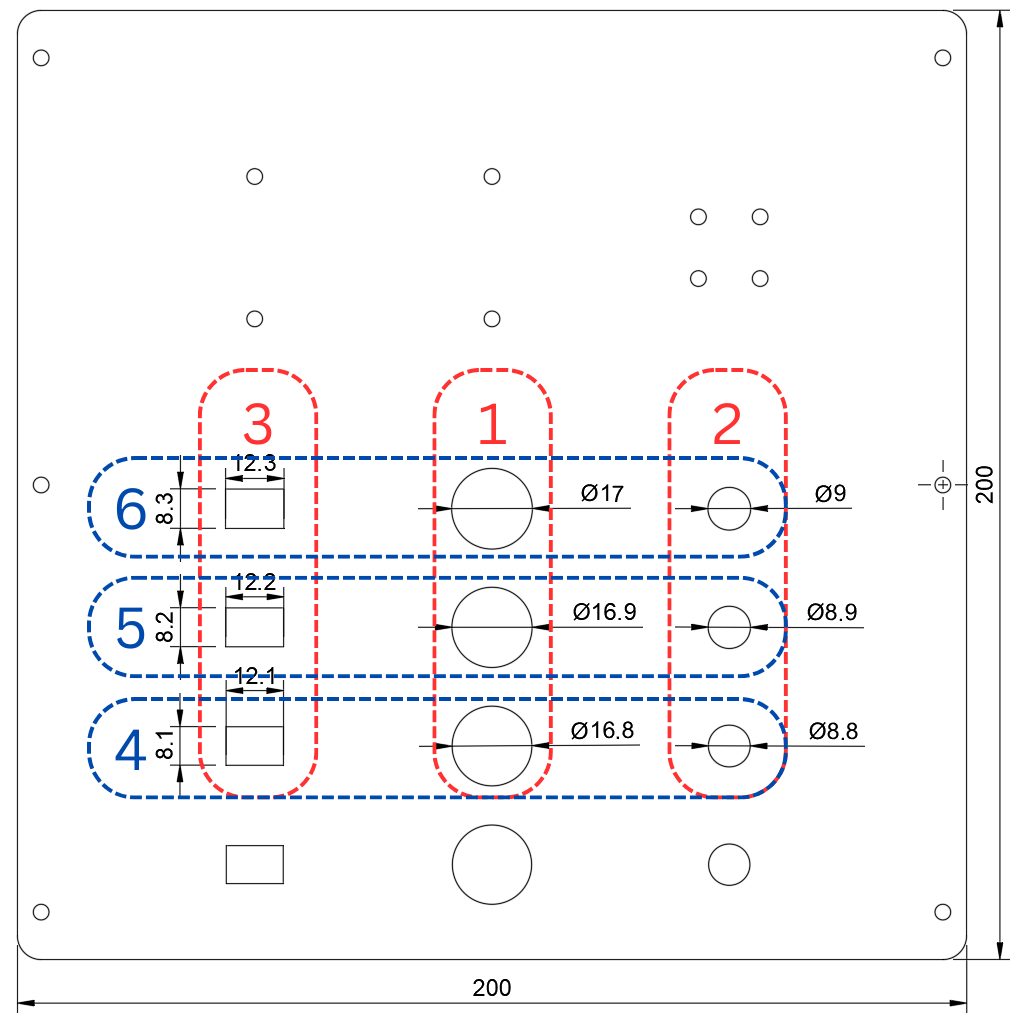
\includegraphics[width=0.6\linewidth]{chapters/6-experiments/bm2_taskboard.png}
    \caption{Held-out group domains used in Benchmark 3. In each case, all sequences belonging to the highlighted group are assigned to the test set. 1: \texttt{BM3\_rod\_geometry\_1} $\dots$ 3: \texttt{BM3\_rod\_geometry\_3}, 4: \texttt{BM3\_tolerance\_1} $\dots$ 6: \texttt{BM3\_tolerance\_3}}
    \label{fig:heldout_groups}
\end{figure}

\newpage

\section{Experiment 3: Deviation Analysis}

\subsection{Motivation}
The dataset recorded in this thesis is not only useful for training a classifier, but the saved metadata alongside each sequence holds valuable information as well, which is useful for further experiments. In particular does each metadata-file hold the information about the exact deviations applied during insertion. This allows the dataset to be analyzed in two ways.
First, as the physical success-rate of insertions is dependent on the applied deviations and their magnitude or level, the goal is to asses which set of deviations, and in particular which level (magnitude), cause more insertion failures than other settings.
But insertion-failure does not imply that the classification model fails to classify the label, for example if the failed insertion produces a clear failure signature, the classifier may be more likely to assign the label "failed insertion" to it. Conversely, a deviation can be physically successful but still produce ambiguous/confusing signal patterns for the classifier. Therefore, the analysis is separated into a physical success-rate analysis and a model-confusion analysis.

\subsection{Deviation Grouping and Domains}
\begin{table}[htbp]
    \centering
    \caption{Deviation parameters available in the dataset.}
    \label{tab:deviation_parameters}
    \begin{tabular}{lll}
        \toprule
        \textbf{Deviation} & \textbf{Level} & \textbf{Interpretation} \\
        \midrule
        Position offset & radial offset in $x,y$-axis & translational misalignment \\
        Tilt & angular deviation around $x,y$-axis & orientational misalignment \\
        Grasp height & 0, 7 mm & grasping configuration \\
        Approach height & -5, 0, 2 mm & vertical approach configuration \\
        Force level & 15, 20, 25, 30, 35, 40 N & commanded insertion force \\
        Force limit & 30, 40, 50 N & contact/force stopping limit \\
        Record offset & -0.2, 0.0, 0.3, 0.6, 0.9 s & temporal recording-window shift \\
        \bottomrule
    \end{tabular}
\end{table}

\tabref{tab:deviation_parameters} shows the available deviation parameters that were applied to the insertions. The exact pattern, how each deviation level got selected for one insertion and how they differ across the recorded batches 1, 2 and 3, are described in detail in the previous Section \ref{sec:dataset_collection}.
In order to more easily report the deviations, the levels of each deviation parameter are combined together in semantic meaningful groups. Because the position offset and tilt are continuous deviations, rather than discrete levels like the Force level, thresholds were selected to assign insertions into semantically meaningful bins.

Before however, the following calculations are necessary.

The position deviation is represented by the Cartesian offsets $\Delta x$ and $\Delta y$ in the insertion plane. These come directly from the \texttt{plan\_item.deviation.x/y} entries in the metadata json file. For the analysis, these values are converted to polar coordinates with radius $r$ and angle $\varphi$ according to

\begin{equation}
    r = \sqrt{\Delta x^2 + \Delta y^2},
    \qquad
    \varphi = \operatorname{atan2}(\Delta y, \Delta x) \bmod 360^\circ .
    \label{eq:polar_coordinates}
\end{equation}

The tilt deviation is represented by the angular deviation angles $\theta_x$ and $\theta_y$ around the $x,y$-axis. They come directly from the \texttt{plan\_item.tilt.x/y} entries in the metadata json file. Its magnitude is computed as

\begin{equation}
    \theta = \sqrt{\theta_x^2 + \theta_y^2}.
    \label{eq:tilt_mag}
\end{equation}

To support the selected thresholds, the distributions of the computed position offset radius $r$ and tilt magnitude $\theta$ are shown in \figref{fig:deviation_threshold_distributions}. The values are sorted in ascending order to visualize how the samples are distributed over the continuous deviation range and where the selected thresholds divide the dataset. The thresholds are not chosen to create equally sized groups, but to form semantically meaningful deviation levels. For the position offset, $r < 0.05~\mathrm{mm}$ is treated as no relevant offset, $0.05~\mathrm{mm} \leq r < 0.25~\mathrm{mm}$ as moderate offset, and $r \geq 0.25~\mathrm{mm}$ as large offset. For the tilt magnitude, $\theta < 0.5^\circ$ is treated as no relevant tilt, $0.5^\circ \leq \theta < 4.0^\circ$ as moderate tilt, and $\theta \geq 4.0^\circ$ as large tilt.

% The resulting group sizes are therefore not expected to be balanced. This is particularly visible for the tilt magnitude, where only a smaller part of the dataset belongs to the no-tilt group. This imbalance reflects the recorded deviation design and is considered in the later analysis by reporting the number of samples per group and by using balanced accuracy for the model-based evaluation.

The following groups in \tabref{tab:deviation_group_definitions} are used for the physical deviation analysis and the model-confusion analysis. Some of these groups are further combined in \tabref{tab:deviation_group_combinations_definitions}, to provide a more in-depth view on the data.

\begin{table}[htbp]
    \centering
    \caption{Definition of deviation groups used for the deviation analysis.}
    \label{tab:deviation_group_definitions}
    \renewcommand{\arraystretch}{1.15}
    \begin{tabular}{p{0.20\textwidth} p{0.31\textwidth} p{0.4\textwidth}}
        \toprule
        \textbf{Deviation group}
        & \textbf{Definition} 
        & \textbf{Group labels} \\
        \midrule

        \texttt{position} 
        & Derived from $r$ as defined in \equref{eq:polar_coordinates}.
        & \texttt{N.O.} (No Offset): $0 \leq r < 0.05~\mathrm{mm}$ \newline
          \texttt{M.O.} (Moderate Offset): $0.05 \leq r < 0.25~\mathrm{mm}$ \newline
          \texttt{L.O.} (Large Offset): $r \geq 0.25~\mathrm{mm}$ \\

        \midrule

        \texttt{tilt} 
        & Derived from $\theta$, the tilt magnitude, as defined in \equref{eq:tilt_mag}.
        & \texttt{N.T.} (No Tilt): $0 \leq \theta < 0.5^\circ$ \newline
          \texttt{M.T.} (Moderate Tilt): $0.5^\circ \leq \theta < 4.0^\circ$ \newline
          \texttt{L.T.} (Large Tilt): $\theta \geq 4.0^\circ$ \\
        \midrule

        \texttt{offset\_direction} 
        & Derived from the polar radius $r$ and angle $\varphi$ as defined in \equref{eq:polar_coordinates}. \figref{fig:offset_direction_sectors} visualizes the selected sectors.
        & \texttt{C}: $r < 0.05~\mathrm{mm}$ \newline
        \texttt{+x}: $315^\circ \leq \varphi < 360^\circ$ or $0^\circ \leq \varphi \leq 45^\circ$ \newline
        \texttt{+y}: $45^\circ < \varphi \leq 135^\circ$ \newline
        \texttt{-x}: $135^\circ < \varphi \leq 225^\circ$ \newline
        \texttt{-y}: $225^\circ < \varphi < 315^\circ$ \\

        \midrule

        \texttt{force\_level} 
        & Commanded insertion force level in Newton.
        & \texttt{F15}, \texttt{F20}, \texttt{F25}, \texttt{F30}, \texttt{F35}, \texttt{F40} \\

        \midrule

        \texttt{force\_limit} 
        & Force threshold used during the insertion attempt.
        & \texttt{L30}, \texttt{L40}, \texttt{L50} \\

        \midrule

        \texttt{record\_offset} 
        & Temporal shift of the recorded signal window. This is not a physical insertion deviation, but changes which part of the insertion process is first visible to the model.
        & \texttt{ROE} (Record Offset Early): $t < 0.1~\mathrm{s}$ \newline
          \texttt{ROM} (Record Offset Mid): $0.1 \leq t < 0.7~\mathrm{s}$ \newline
          \texttt{ROL} (Record Offset Late): $0.7 \leq t~\mathrm{s}$ \\

        \midrule

        \texttt{grasp\_height} 
        & Height offset used during grasping.
        & \texttt{0}, \texttt{7}\\

        \midrule

        \texttt{approach\_height} 
        & Height offset used during the approach motion before insertion.
        & \texttt{-5}, \texttt{0}, \texttt{2}\\

        \bottomrule
    \end{tabular}
\end{table}

\begin{figure}[htbp]
    \centering
    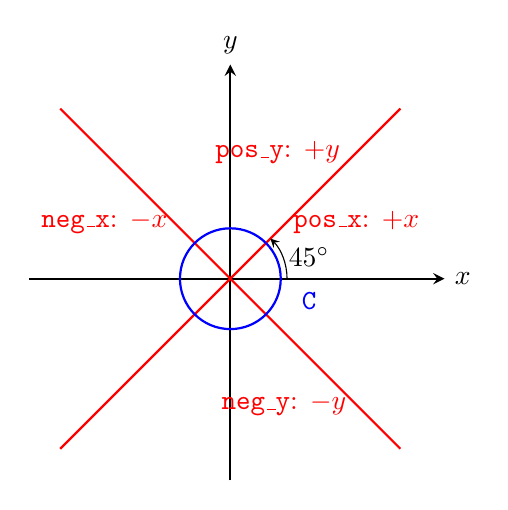
\begin{tikzpicture}[scale=0.8, >=stealth]

        % Axes
        \draw[->, thick] (-3.2,0) -- (3.4,0) node[right] {$x$};
        \draw[->, thick] (0,-3.2) -- (0,3.4) node[above] {$y$};

        % Sector boundaries
        \draw[red, thick] (-2.7,-2.7) -- (2.7,2.7);
        \draw[red, thick] (-2.7,2.7) -- (2.7,-2.7);

        % Centered circle
        \draw[blue, thick] (0,0) circle (0.8);
        \node[blue] at (1.25,-0.35) {\texttt{C}};

        % Sector labels
        \node[red] at (2.0,0.9) {\texttt{pos\_x}: $+x$};
        \node[red] at (-2.0,0.9) {\texttt{neg\_x}: $-x$};
        \node[red] at (0.75,2.0) {\texttt{pos\_y}: $+y$};
        \node[red] at (0.85,-2.0) {\texttt{neg\_y}: $-y$};

        % Angle annotation
        \draw[->] (0.9,0) arc[start angle=0,end angle=45,radius=0.9];
        \node at (1.25,0.35) {$45^\circ$};

    \end{tikzpicture}
    \caption{Definition of offset-direction sectors in the insertion plane. Samples inside the centered region are assigned to \texttt{C}. Outside this region, the polar angle and radius determine whether the sample belongs to the positive or negative $x$/$y$ sector.}
    \label{fig:offset_direction_sectors}
\end{figure}

\begin{table}[htbp]
    \centering
    \caption{Definition of combined deviation groups used for the deviation analysis.}
    \label{tab:deviation_group_combinations_definitions}
    \renewcommand{\arraystretch}{1.15}
    \begin{tabular}{p{0.2\textwidth} p{0.25\textwidth} p{0.47\textwidth}}
        \toprule
        \textbf{Deviation group}
        & \textbf{Definition} 
        & \textbf{Group labels} \\
        \midrule

        \texttt{position\_tilt} 
        & Combination of the position-offset level and the tilt-magnitude level.
        & (\texttt{N.O. / N.T.}), (\texttt{N.O. / M.T.}), (\texttt{N.O. / L.T.}),\newline
        (\texttt{M.O. / N.T.}), (\texttt{M.O. / M.T.}), (\texttt{M.O. / L.T.}),\newline
        (\texttt{L.O. / N.T.}), (\texttt{L.O. / M.T.}), (\texttt{L.O. / L.T.})\\

        \midrule

        \texttt{force\_interaction} 
        & Combination of force level and force limit. This group is used because the effect of the force limit depends on the force level.
        & (\texttt{F15 / L30}), (\texttt{F15 / L40}), (\texttt{F15 / L50}),\newline
        (\texttt{F20 / L300}), (\texttt{F20 / L40}), (\texttt{F20 / L50}),\newline
        (\texttt{F25 / L30}), (\texttt{F25 / L40}), (\texttt{F25 / L50}),\newline
        (\texttt{F30 / L30}), (\texttt{F30 / L40}), (\texttt{F30 / L50}),\newline
        (\texttt{F35 / L30}), (\texttt{F35 / L40}), (\texttt{F35 / L50}),\newline
        (\texttt{F40 / L30}), (\texttt{F40 / L40}), (\texttt{F40 / L50})\\

        \bottomrule
    \end{tabular}
\end{table}

\begin{figure}[htbp]
    \centering
    \begin{subfigure}[t]{0.45\textwidth}
        \centering
        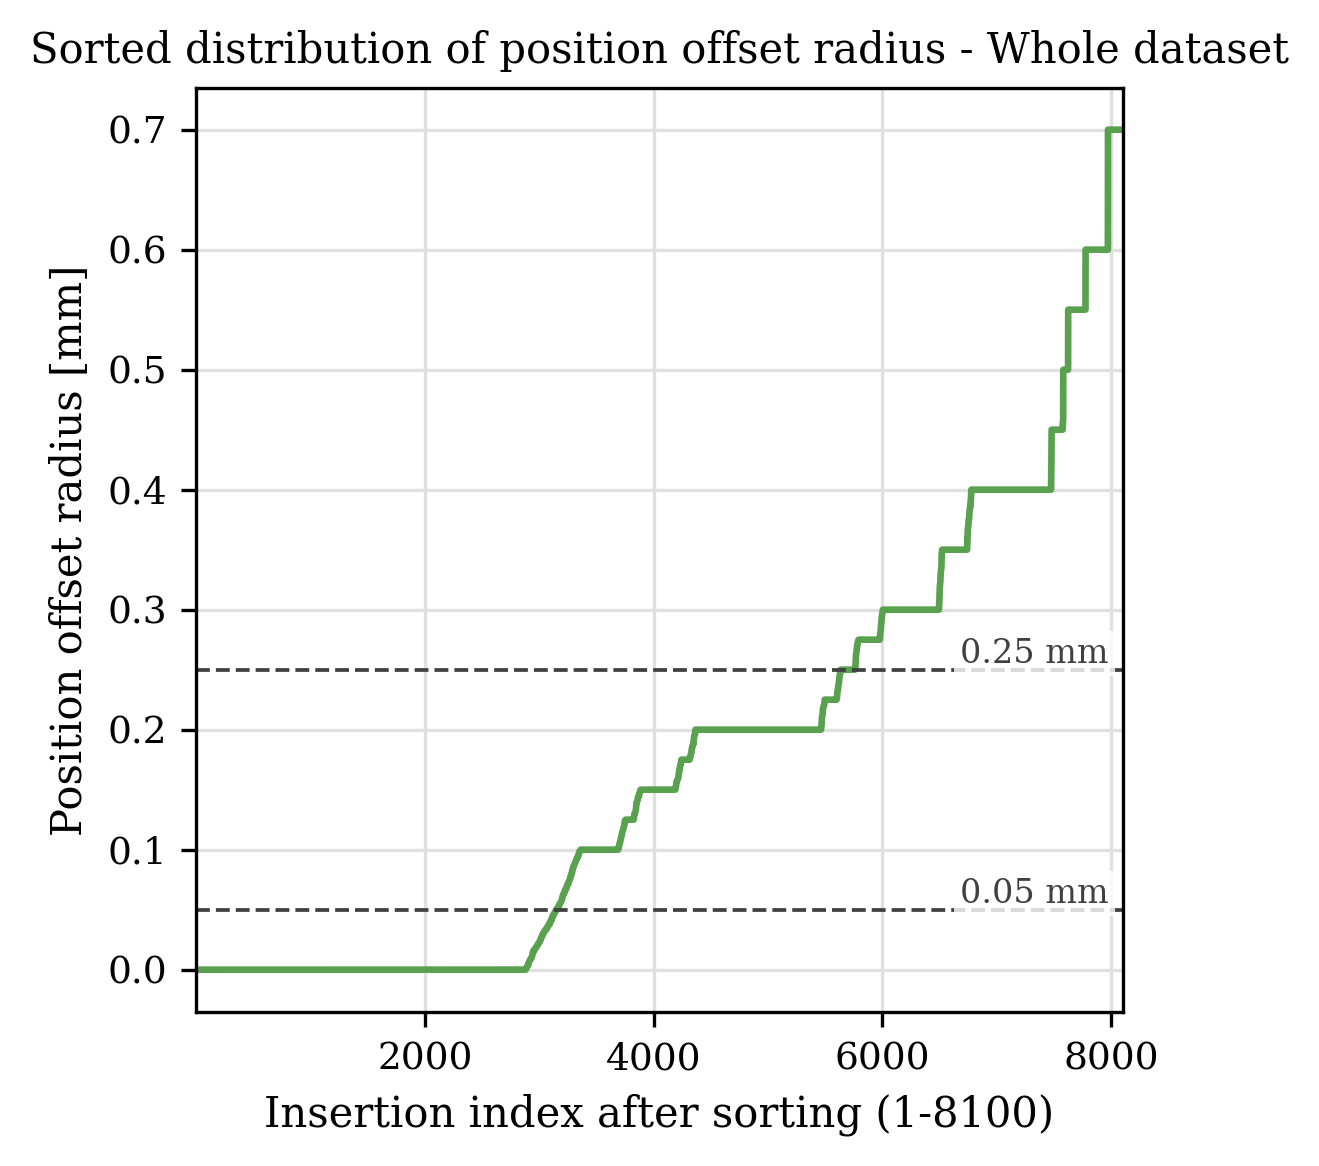
\includegraphics[width=0.95\textwidth]{chapters/6-experiments/sorted_radius_mm_distribution.png}
        \caption{Sorted distribution of position offset radius $r$.}
        % \label{fig:sorted_radius_distribution}
    \end{subfigure}
    \begin{subfigure}[t]{0.45\textwidth}
        \centering
        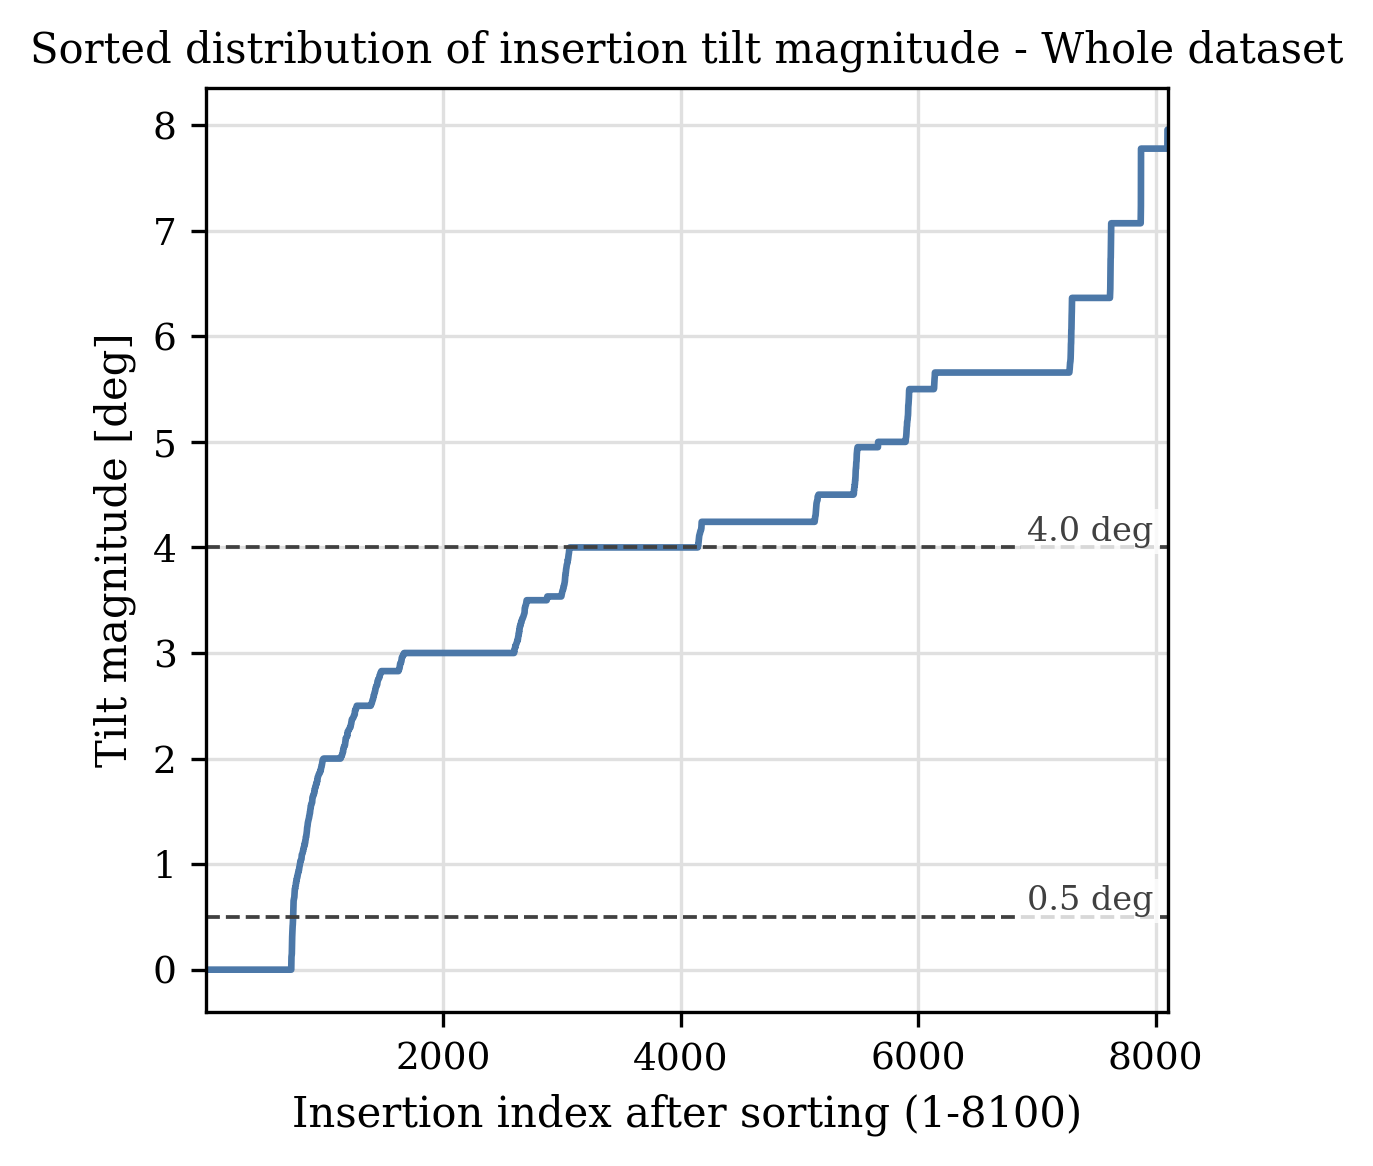
\includegraphics[width=0.99\textwidth]{chapters/6-experiments/sorted_tilt_mag_deg_distribution.png}
        \caption{Sorted distribution of tilt magnitude $\theta$.}
        % \label{fig:sorted_tilt_distribution}
    \end{subfigure}

    \caption{Sorted distributions of the continuous position and tilt deviations used for defining the deviation groups. Dashed lines indicate the thresholds used to assign samples to the no, moderate, and large deviation levels.}
    \label{fig:deviation_threshold_distributions}
\end{figure}

To summarize, the deviation group and the domain are two different ways to index the metadata and select a specific subset of the whole dataset. The deviation group concentrates on how the rod was inserted, what deviations were present. These settings changed with each consecutive insertion attempt. Whereas the domain selects a subset based on the physical properties and experimental configuration, such as rod type, batch, tolerance, and gripper type. These settings change after each recording session.

\subsection{Deviation Analysis I: Physical Success Rate}
\label{sec:deviation_analysis_physical}

The first part of the deviation analysis investigates how the physical insertion outcome is distributed across the deviation groups defined in \tabref{tab:deviation_group_definitions} and \tabref{tab:deviation_group_combinations_definitions}. This analysis is based only on the metadata files and does not use any model predictions. For each selected domain subset of the dataset, the number of successful and failed insertions for each deviation group within the selected domain is counted. The physical success rate is then computed for each deviation group as

\begin{equation}
    r_\mathrm{success}
    =
    \frac{N_\mathrm{success}}
    {N_\mathrm{success} + N_\mathrm{failure}} .
    \label{eq:physical_success_rate}
\end{equation}

The analysis is first performed on the complete dataset, with all domain attributes are set to \texttt{None}. Thus, no restriction is applied to \texttt{batch}, \texttt{rod\_type}, \texttt{tolerance}, or \texttt{gripper\_type}. This global analysis provides a first overview of which deviation groups are generally associated with more successful or failed insertions.

Afterwards, the same analysis is repeated for domain-specific subsets. These subsets are created by fixing one or multiple domain attributes, for example a specific hole domain such as \texttt{rect\_rod} with tolerance \texttt{0.1}, or a broader domain such as all samples with \texttt{tolerance = 0.2}. This allows the physical success rate of a deviation group to be evaluated not only globally, but also in relation to specific rods, tolerances, grippers, or batches. This is important because the dataset is not a fully balanced experiment and because the deviation design differs between batches.

The physical success-rate analysis is performed for the individual deviation groups, such as \texttt{position}, \texttt{tilt}, \texttt{offset\_direction}, \texttt{force\_level}, \texttt{force\_limit}, \texttt{grasp\_height}, and \texttt{approach\_height}, as well as for selected combined groups such as \texttt{position\_tilt} and \texttt{force\_interaction}. The \texttt{record\_offset} group is also evaluated descriptively, but it is not interpreted as a physical cause of insertion success or failure, because it only changes the temporal position of the recorded signal window.

Due to the large number of possible deviation-domain combinations, not every generated table or plot is reported in the results chapter. Instead, the results focus on the most informative comparisons, namely deviation groups that show clear differences in physical success rate, systematic trends across levels, or notable domain-specific behavior.

\subsection{Deviation Analysis II: Model Confusion}
\label{sec:deviation_analysis_model_confusion}

The second part of the deviation analysis investigates whether the classification model shows systematic error patterns for specific deviation groups. It evaluates how well the trained model classifies samples belonging to different deviation groups.

For this analysis, the PatchTST model is trained 9 times according to Section \ref{sec:reporing_of_experiments} and evaluated using the standard mixed train-validation-test procedure, already presented for Benchmark 1. The test set therefore contains samples from the same overall dataset distribution as the training data.

During test-set evaluation, one prediction record is saved for every tested sample. Each record contains the true label, predicted probability, predicted class, correctness, binary cross-entropy loss, the corresponding metadata values, the assigned deviation groups, and the domain attributes. The predicted class is obtained using the optimized threshold of the respective training run. This is important because the decision threshold is not fixed at 0.5, but selected from the validation data.

The model-confusion analysis is first performed globally, again corresponding to the domain selection where all domain attributes are set to \texttt{None}. The test predictions are grouped by the same deviation groups used in Deviation Analysis I. For each deviation group, the following metrics are computed:

\begin{itemize}
    \item balanced accuracy,
    \item binary cross-entropy loss,
    \item false-positive rate,
    \item false-negative rate.
\end{itemize}

Balanced accuracy is used as the main classification metric because individual deviation groups can contain unequal numbers of successful and failed insertions. The binary cross-entropy loss is used to identify cases where the model assigns strongly incorrect probabilities. The false-positive and false-negative rates show whether the model tends to confuse failed insertions with successful ones or the other way around.

As in Deviation Analysis I, the model-confusion analysis is then repeated for domain-specific subsets. This allows the same deviation group to be evaluated for specific rods, tolerances, grippers, or batches. The resulting domain-specific analysis is used to check whether model confusion is a global property of a deviation group or whether it mainly occurs in specific dataset domains.

Only the most relevant model-confusion results are selected for the results chapter. These include deviation groups with low balanced accuracy, high loss, low confidence, or notable false-positive or false-negative tendencies.\\\\
Furthermore, cases where physical difficulty and model difficulty differ, are highlighted as well, because a deviation group can be physically difficult but easy for the model to classify if it produces clear failure signatures. On the other hand, a deviation group can have a high physical success rate but still be model-confusing if the signal patterns are ambiguous.

